\documentclass[5p,times,authoryear]{elsarticle}
\usepackage[T1]{fontenc}
\usepackage[utf8]{inputenc}
\PassOptionsToPackage{hyphens}{url}
\usepackage[table]{xcolor}
\definecolor{WETNavy}{HTML}{1B3765}
\definecolor{WETTeal}{HTML}{0B5563}
\definecolor{WETCrimson}{HTML}{E11D48}
\definecolor{WETSlate}{HTML}{334155}
\usepackage{amsmath,amssymb,booktabs,graphicx,microtype,url,placeins,float,multirow,tabularx,array,balance}
\usepackage[colorlinks=true,citecolor=WETNavy,linkcolor=WETNavy,urlcolor=WETTeal]{hyperref}
\graphicspath{{figures/}{figures/appendix/}}
\setlength{\dbltextfloatsep}{8pt plus 2pt minus 2pt}
\setlength{\textfloatsep}{8pt plus 2pt minus 2pt}
\setlength{\intextsep}{8pt plus 2pt minus 2pt}
\emergencystretch=1.5em
\newcommand{\usdps}{\texttt{Usd\allowbreak Preview\allowbreak Surface}}
\newcommand{\original}{\textsc{Original}}
\newcommand{\converted}{\textsc{Converted}}
\newcommand{\OurStudy}{paired material intervention}

\newcommand{\NavN}{99}
\newcommand{\NavFlips}{30}
\newcommand{\NavFlipPercent}{30.3}
\newcommand{\NavSrOriginal}{52.5}
\newcommand{\NavSrConverted}{48.5}
\newcommand{\NewRunCount}{12}
\newcommand{\BoardCount}{4}
\newcommand{\GemmaFullOrig}{12}
\newcommand{\GemmaFullOrigPercent}{75.0}
\newcommand{\GemmaFullConv}{13}
\newcommand{\GemmaFullConvPercent}{81.2}
\newcommand{\GemmaFullFlips}{3}
\newcommand{\GemmaActionOrig}{12}
\newcommand{\GemmaActionOrigPercent}{75.0}
\newcommand{\GemmaActionConv}{12}
\newcommand{\GemmaActionConvPercent}{75.0}
\newcommand{\GemmaActionFlips}{2}
\newcommand{\GemmaTargetOrig}{12}
\newcommand{\GemmaTargetOrigPercent}{75.0}
\newcommand{\GemmaTargetConv}{11}
\newcommand{\GemmaTargetConvPercent}{68.8}
\newcommand{\GemmaTargetFlips}{3}
\newcommand{\GemmaContextOrig}{12}
\newcommand{\GemmaContextOrigPercent}{75.0}
\newcommand{\GemmaContextConv}{14}
\newcommand{\GemmaContextConvPercent}{87.5}
\newcommand{\GemmaContextFlips}{2}
\newcommand{\SmallFullOrig}{14}
\newcommand{\SmallFullOrigPercent}{87.5}
\newcommand{\SmallFullConv}{14}
\newcommand{\SmallFullConvPercent}{87.5}
\newcommand{\SmallFullFlips}{2}
\newcommand{\SmallActionOrig}{9}
\newcommand{\SmallActionOrigPercent}{56.2}
\newcommand{\SmallActionConv}{12}
\newcommand{\SmallActionConvPercent}{75.0}
\newcommand{\SmallActionFlips}{3}
\newcommand{\SmallTargetOrig}{14}
\newcommand{\SmallTargetOrigPercent}{87.5}
\newcommand{\SmallTargetConv}{15}
\newcommand{\SmallTargetConvPercent}{93.8}
\newcommand{\SmallTargetFlips}{3}
\newcommand{\SmallContextOrig}{14}
\newcommand{\SmallContextOrigPercent}{87.5}
\newcommand{\SmallContextConv}{16}
\newcommand{\SmallContextConvPercent}{100.0}
\newcommand{\SmallContextFlips}{2}
\newcommand{\LargeFullOrig}{16}
\newcommand{\LargeFullOrigPercent}{100.0}
\newcommand{\LargeFullConv}{15}
\newcommand{\LargeFullConvPercent}{93.8}
\newcommand{\LargeFullFlips}{1}
\newcommand{\LargeActionOrig}{15}
\newcommand{\LargeActionOrigPercent}{93.8}
\newcommand{\LargeActionConv}{15}
\newcommand{\LargeActionConvPercent}{93.8}
\newcommand{\LargeActionFlips}{0}
\newcommand{\LargeTargetOrig}{16}
\newcommand{\LargeTargetOrigPercent}{100.0}
\newcommand{\LargeTargetConv}{15}
\newcommand{\LargeTargetConvPercent}{93.8}
\newcommand{\LargeTargetFlips}{1}
\newcommand{\LargeContextOrig}{16}
\newcommand{\LargeContextOrigPercent}{100.0}
\newcommand{\LargeContextConv}{16}
\newcommand{\LargeContextConvPercent}{100.0}
\newcommand{\LargeContextFlips}{0}

\journal{Computer Vision and Image Understanding}
\begin{document}
\begin{frontmatter}
\title{Geometric Fidelity Is Not Decision Fidelity: Bidirectional Optical Turnover and Pre-Deployment Risk Gating Under 3D Material Conversion}
\author[shlab]{Zihou Zhu\corref{cor1}}
\ead{zhuzihou@pjlab.org.cn}
\cortext[cor1]{Corresponding author.}
\address[shlab]{Shanghai Artificial Intelligence Laboratory, Shanghai, China}
\begin{abstract}
Cross-simulator 3D asset reuse routinely lowers vendor-specific material definitions---here translating NVIDIA Material Definition Language (\textsc{MDL}) networks into portable \usdps{} shaders---while leaving scene meshes, camera poses, and language instructions invariant. Across 30 indoor scenes (240 objects, 480 paired captures, 14,016 total \textsc{VLM} predictions) and a 99-episode closed-loop navigation study, we find that geometric invariance does not guarantee decision invariance, and that dataset-level accuracy conceals substantial bidirectional decision turnover. Across four independent open-weight \textsc{VLM} families spanning six checkpoints---\textsc{Qwen3-VL} (2B, 8B, 32B), \textsc{InternVL3.5-8B-HF}, \textsc{Molmo2-8B} (SigLIP-2), and \textsc{LLaVA-NeXT-Mistral-7B} (Mistral-7B + CLIP)---net hit-rate shifts remain modest ($+0.42\%$ on 32B, \textsc{Molmo2-8B}, and \textsc{LLaVA-NeXT}; $+1.46\%$ to $+1.88\%$ on 8B), yet $4.17\%$ to $23.13\%$ of individual localizations reverse pass/fail status across shader conditions. A four-level variance hierarchy isolates this effect from runtime and rendering noise: deterministic greedy decoding yields $0.00\%$ ($0.00\,\mathrm{px}$) repeat disagreement across all six checkpoints, whereas material conversion induces $2.00\times$ to $6.00\times$ more decision flips than same-material ray-tracing re-renders ($4.17\%$ vs.\ $0.00\%$ on \textsc{Molmo2-8B}), while stochastic decoding ($T{=}0.2$) introduces an $8.96\%$ pairwise ($16.67\%$ any-flip) noise floor. Evaluating 2,880 pixel-exact silhouette counterfactuals and $\mathrm{CIE}~L^*a^*b^*$ photometric controls across both \textsc{Qwen3-VL-8B} and \textsc{InternVL3.5-8B-HF} reveals an identical $+3.54\%$ non-photometric \textsc{BSDF} residual ($+3.38\%$ on bit-identical masks) above affine luminance and color matching, reflecting a mechanism trade-off in which glare removal assists metallic targets while surface flattening impairs subtle cues. Because $85.7\%$ of $\ge$7B regressions are specific to a single architecture, a family-calibrated zero-\textsc{VLM} risk gate trained on mask geometry and paired appearance deltas predicts directional \textsc{Qwen3-VL} losses (\textsc{AUROC} $= 0.743$ held-out test, $0.732$ 30-scene \textsc{LOSO}), recovering $52.0\%$ of \textsc{LOSO} regressions within a $20\%$ review budget where global \textsc{RGB MAE} fails ($0.432$).

\end{abstract}
\begin{keyword}visual grounding \sep 3D material conversion \sep vision-language models \sep counterfactual diagnosis \sep embodied simulation\end{keyword}
\begin{highlights}
\item 3D shader lowering flips 4.2--23.1\% of VLM decisions despite small net shifts.
\item Turnover exceeds 0.0\% greedy and ray noise across 4 VLM families.
\item 2,880 counterfactuals reveal a +3.54\% non-photometric BSDF residual.
\item Glare removal aids metallic targets (+4.4\%) while glass and texture cues regress.
\item A zero-VLM geometry gate reaches 0.743 AUROC where global RGB MAE fails (0.432).
\end{highlights}
\end{frontmatter}
\section{Introduction}
\label{sec:intro}

Simulation pipelines for embodied artificial intelligence routinely port 3D environments across rendering engines, physics backends, and dataset repositories. During asset ingestion and cross-platform export, proprietary shader graphs authored in NVIDIA Material Definition Language (\textsc{MDL}) within Universal Scene Description (\textsc{USD}) archives are commonly lowered into portable \usdps{} networks. This translation leaves triangle meshes, object poses, articulation hierarchies, camera intrinsics, and language goals untouched. Geometrically, the converted scene appears exact; visually, surface reflectance, specular highlights, glass transmission, local edge contrast, and indirect illumination shift together. Quantifying how this routine conversion alters Vision-Language Model (\textsc{VLM}) decisions is essential before converted assets can be relied upon in evaluation or sim-to-real pipelines.

Benchmarking converted assets by dataset-level accuracy alone hides a critical reliability failure. In many scenes, degraded glass highlights or flattened surface texture cause a model to miss targets it previously grounded, while a comparable number of glare-occluded metallic objects become easier to localize. Their net difference nearly cancels in aggregate accuracy ($+0.42\%$ on \textsc{Qwen3-VL-32B}, \textsc{Molmo2-8B}, and \textsc{LLaVA-NeXT-Mistral-7B}), even as $4.17\%$ to $23.13\%$ of individual task outcomes reverse between conditions. For safety-critical inspection and downstream closed-loop embodied control, silent regression on previously solved instances cannot be offset by incidental improvements elsewhere.

\begin{figure*}[!t]
\centering
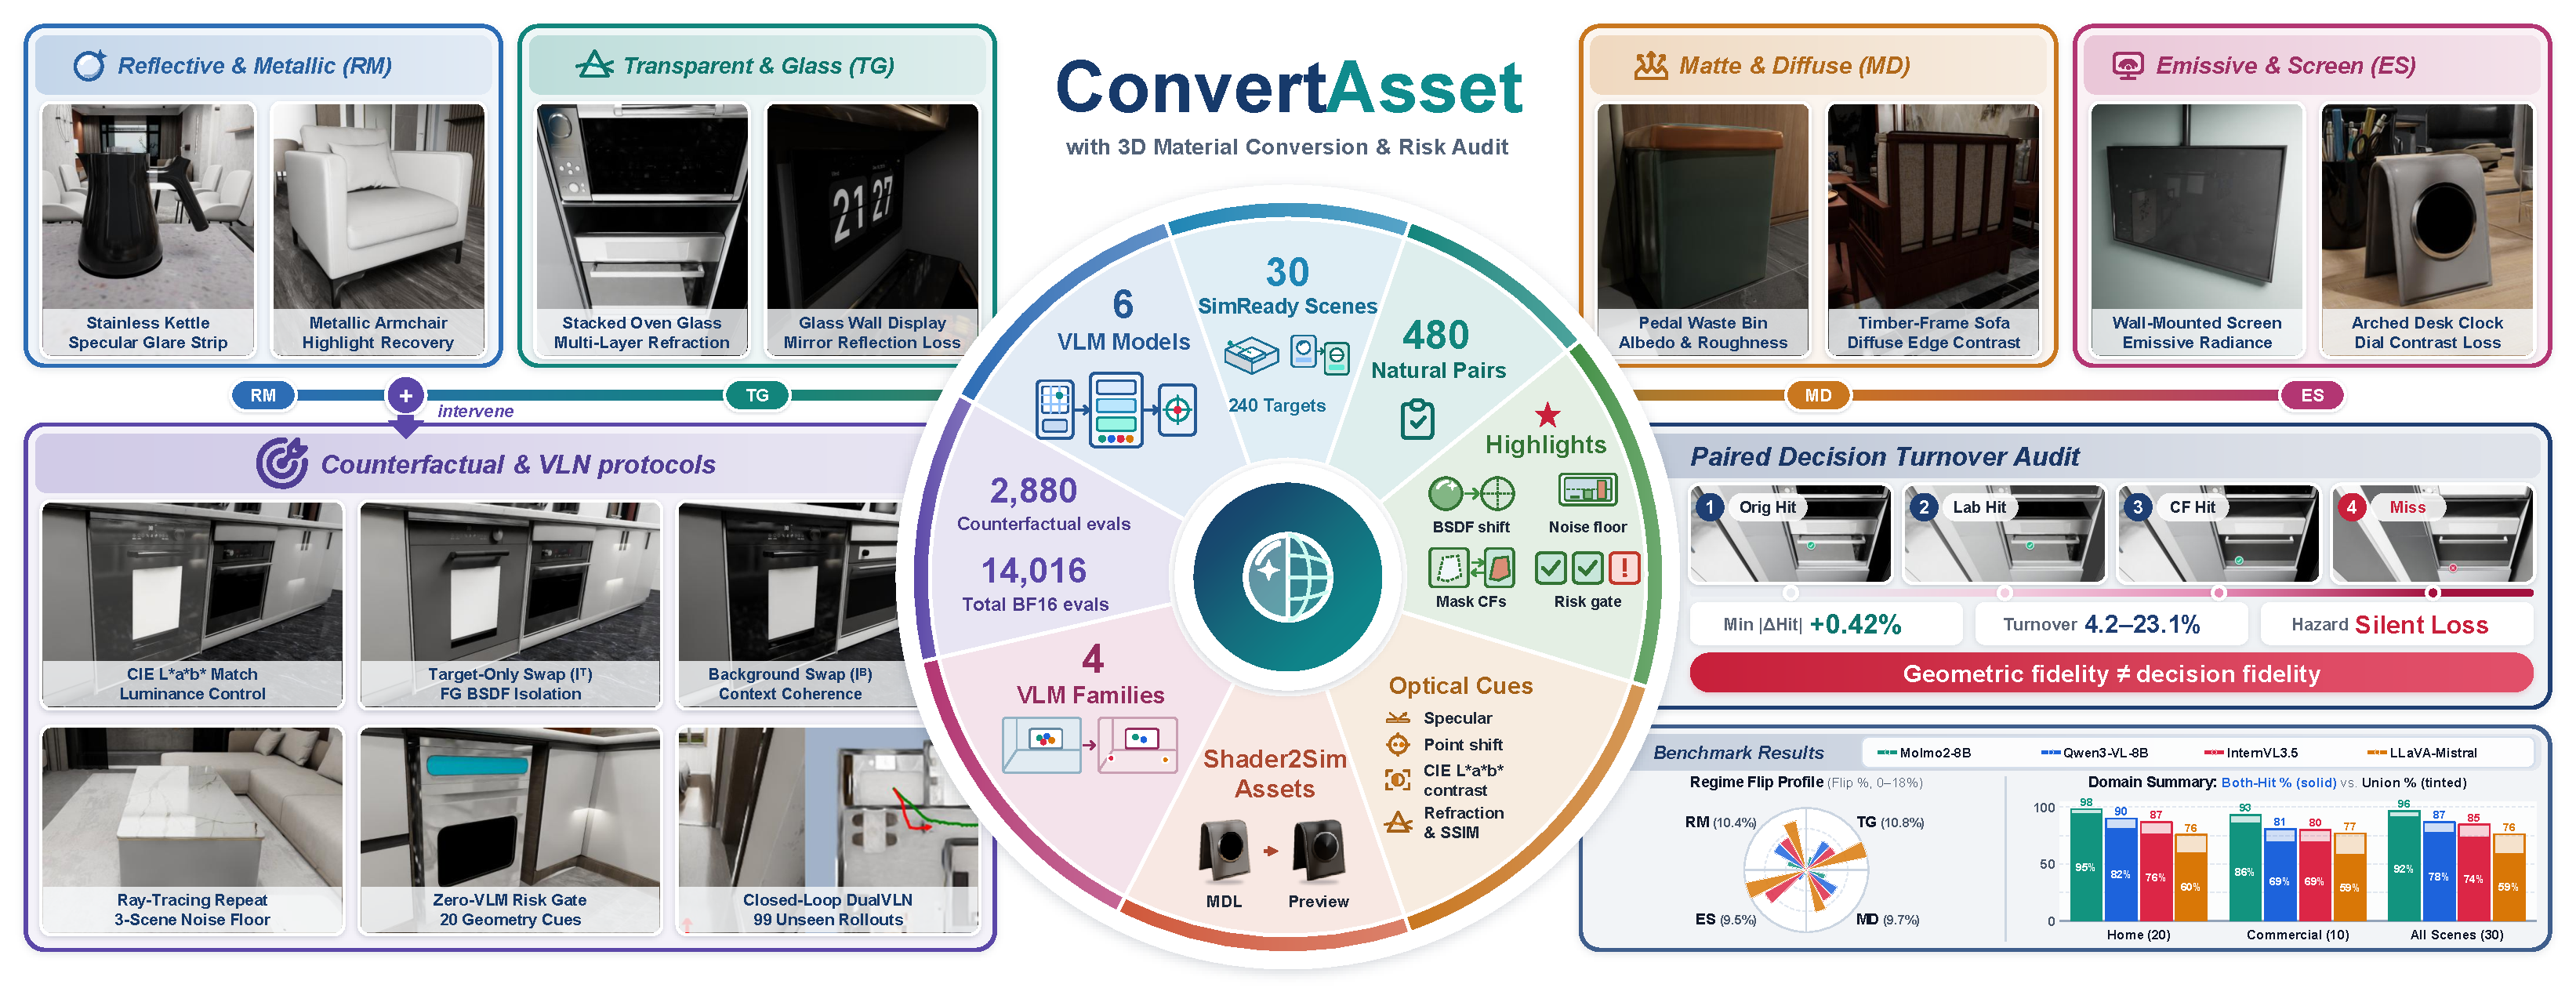
\includegraphics[width=\textwidth]{fig1_overview.pdf}
\caption{\textbf{Overview of the \textsc{ConvertAsset} benchmark, optical domain taxonomy, counterfactual protocols, and four-family audit.}
Across 30 geometry-locked SimReady scenes (240 targets, 480 natural pairs) and four open-weight \textsc{VLM} families under deterministic inference, lowering NVIDIA \textsc{MDL} shaders to \texttt{UsdPreviewSurface} induces $4.2\text{--}23.1\%$ bidirectional pass/fail decision turnover despite small marginal hit-rate deltas ($\min |\Delta H| = +0.4\%$). \emph{Top corners:} paired optical examples spanning Reflective \& Metallic (\textsc{RM}), Transparent \& Glass (\textsc{TG}), Matte \& Diffuse (\textsc{MD}), and Emissive \& Screen (\textsc{ES}). \emph{Bottom:} pixel-exact counterfactual protocols (2,880 evaluations), zero-\textsc{VLM} risk gate, 99 closed-loop \textsc{VLN} episodes, and four-family regime flip profiles and consistency gaps.}
\label{fig:overview}
\end{figure*}

Three methodological gaps limit prior robustness work when applied to 3D asset conversion (Section~\ref{sec:related}). First, classical corruption benchmarks apply 2D post-processing noise or style transfer \citep{Geirhos2019Texture,Hendrycks2019Benchmarking}, whereas generative editing benchmarks modify object silhouettes alongside surface appearance \citep{Zhang2024ImageNetD}. Second, spatial grounding evaluations frequently entangle appearance sensitivity with coordinate-frame mismatches (pixels vs.\ normalized $0\text{--}1000$ outputs), decoding randomness \citep{Zhao2021Calibrate}, and path-tracing noise, obscuring whether shader effects exceed runtime variance. Third, conventional pixel metrics such as global \textsc{RGB MAE} penalize helpful glare reduction symmetrically with damaging contrast loss, offering little guidance on which converted scenes merit manual inspection.

Figure~\ref{fig:overview} outlines our end-to-end empirical framework. Within \textsc{ConvertAsset}, we hold scene graphs, meshes, transforms, and camera viewpoints identical between \textsc{MDL} (\original) and \usdps{} (\converted) renders across 30 indoor scenes (20 residential, 10 commercial; 240 visible target instances across 480 camera views). Using calibrated deterministic readout protocols validated via an independent coordinate-format qualification step (\ref{app:readout}), we examine four open-weight \textsc{VLM} families (\textsc{Qwen3-VL}, \textsc{InternVL3.5}, \textsc{Molmo2}, and \textsc{LLaVA-NeXT-Mistral}) along four axes:
\begin{itemize}
    \item \textbf{RQ1 (Variance Floor, Scaling, and Four-Family Generality):} Does material-induced bidirectional turnover exceed greedy runtime repeatability and path-tracing variance across all six checkpoints, a $16\times$ parameter span (\textsc{Qwen3-VL-2B/8B/32B}), and four distinct architectures?
    \item \textbf{RQ2 (Cross-Family Causal Optical Mechanisms):} Across 2,880 pixel-exact silhouette counterfactuals and $\mathrm{CIE}~L^*a^*b^*$ photometric controls on two independent 8B architectures, how much turnover arises from overall luminance and color shifts versus non-photometric Bidirectional Scattering Distribution Function (\textsc{BSDF}) structure?
    \item \textbf{RQ3 (Pre-Deployment Risk Gating):} Can lightweight target-geometry and paired-render cues flag conversion regressions prior to running any \textsc{VLM}, outperforming global \textsc{RGB MAE}, and how does cross-architecture regression divergence affect family-specific versus pooled risk gates?
    \item \textbf{RQ4 (Downstream Embodied Control):} How does paired material conversion manifest in sequential closed-loop Vision-and-Language Navigation (\textsc{VLN}) over 99 unseen apartment episodes?
\end{itemize}

\paragraph{Summary of contributions}
\begin{enumerate}
    \item \textbf{Four-Family Asset-Conversion Benchmark and Noise Floor (Sections~\ref{sec:method}--\ref{sec:grounding}):} Across 14,016 deterministic predictions spanning 4 \textsc{VLM} families and 6 checkpoints over 30 scenes, small marginal deltas ($+0.42\%$ on 32B, \textsc{Molmo2-8B}, and \textsc{LLaVA-NeXT}) conceal $4.17\%\text{--}23.13\%$ bidirectional flips. Greedy repeatability stays at $0.00\%$ ($0.00\,\mathrm{px}$) on every checkpoint, whereas shader conversion exceeds same-material ray-tracing variance by $2.00\times$ to $6.00\times$ ($4.17\%$ vs.\ $0.00\%$ on \textsc{Molmo2-8B}).
    \item \textbf{Cross-Family Causal Silhouette Counterfactuals (Section~\ref{sec:mechanisms}):} Across 2,880 counterfactual evaluations on \textsc{Qwen3-VL-8B} and \textsc{InternVL3.5-8B-HF}, both architectures retain an identical \textbf{$+3.54\%$} non-photometric shader residual above $\mathrm{CIE}~L^*a^*b^*$ salience matching ($+3.38\%$ on the 473 bit-identical mask subset), reflecting glare cleanup on metallic objects balanced against glass and texture degradation.
    \item \textbf{Family-Calibrated vs.\ Pooled Risk Gating (Section~\ref{sec:risk_gate}):} An $\ell_2$-regularized logistic gate combining target geometry with paired appearance deltas reaches $0.743$ held-out test \textsc{AUROC} ($0.732$ 30-scene \textsc{LOSO}) on \textsc{Qwen3-VL} regressions, capturing $52.0\%$ of \textsc{LOSO} losses within a $20\%$ inspection budget where global \textsc{RGB MAE} yields $0.432$. Finding that $85.7\%$ ($66/77$) of $\ge$7B losses are unique to a single architecture further explains why pre-deployment gates must be calibrated per model family ($0.582$ test / $0.536$ \textsc{LOSO} when pooled).
    \item \textbf{Downstream Closed-Loop Context and Analysis Suite (Section~\ref{sec:navigation}):} We extend the static grounding analysis with 99 paired closed-loop \textsc{InternNav/\allowbreak DualVLN} episodes showing $30.3\%$ episode-outcome turnover, alongside a complete set of scene renders, mask counterfactuals, and diagnostic scripts.
\end{enumerate}

\paragraph{Relation to preliminary workshop work}
A preliminary workshop study introducing the underlying conversion toolkit appeared in \citet{Zhu2026Evaluating}, focusing on single-asset image similarity (\textsc{PSNR}, \textsc{SSIM}, \textsc{LPIPS}), feature cosines (\textsc{CLIP}, \textsc{DINOv2}), and simulator warm-up timing. Over $85\%$ of the present article is new, contributing the 30-scene \textsc{ConvertAsset} grounding benchmark, 14,016 four-family \textsc{VLM} evaluations, the four-level variance hierarchy, 2,880 silhouette counterfactuals, family-calibrated zero-\textsc{VLM} risk gating, and the 99-episode closed-loop navigation study.

\section{Related Work}
\label{sec:related}

Our work sits at the intersection of visual appearance robustness, counterfactual \textsc{VLM} diagnosis, and 3D embodied simulation. Table~\ref{tab:related_work} summarizes how our protocol differs from prior literature.

\begin{table*}[!t]
\centering\scriptsize
% Prior robustness/bias benchmarks compared with ConvertAsset
\begin{tabular*}{\textwidth}{@{\extracolsep{\fill}}p{3.1cm}p{3.0cm}p{3.2cm}p{2.9cm}p{3.7cm}@{}}
\toprule
Work & Stimulus / Domain & Perturbation Mechanism & Primary Metrics & Key Distinction vs.\ Ours \\
\midrule
\citet{Geirhos2019Texture}; \citet{Burgert2025NotTexture} & 2D ImageNet categories & Neural style transfer or post-hoc cue suppression & Top-1 acc., shape vs.\ texture ratio & We keep geometry fixed via 3D shader conversion on indoor scenes. \\
\citet{Hendrycks2019Benchmarking} & ImageNet-C / -P corruptions & Additive 2D pixel noise, blur, weather, digital & mCE, flip prob.\ on frame sequences & Our converted renders stay clean (1024$\times$768) with zero sensor corruption. \\
\citet{Zhang2024ImageNetD} & Diffusion synthetic objects & Unconstrained generative backgrounds/textures & Classification accuracy drop & Deterministic USD shader mapping avoids generative shape drift. \\
\citet{Gavrikov2025Talk}; \citet{Eppel2025Shape} & 2D/3D cue-conflict \& LAS\&T & Prompt steering; multi-factor crop variation & Category / material accuracy & Fixed pointing prompt measuring pixel-exact localization turnover. \\
\citet{Tong2024EyesWideShut}; \citet{Sar2026RealityCheck} & MMVP; Reality Check VQA & CLIP-blind pairs; 2D edit / swap counterfactuals & VQA accuracy across bias axes & Native 3D BSDF swaps paired with $\mathrm{CIE}~L^*a^*b^*$ salience matching. \\
\citet{Wang2026ConstantEye} & \emph{navdream} driving & Generative pixel-aligned style transfer & Driving trajectories \& adapter stability & Indoor SimReady MDL$\to$Preview conversion across 4 VLM families + risk gating. \\
\citet{Chaubey2020UAP} & Adversarial robustness survey & Gradient-optimized universal pixel noise & Attack success / fooling rate & Unoptimized engineering export induces bidirectional gains and losses. \\
\midrule
\textbf{Ours (\textsc{ConvertAsset})} & \textbf{30 USD scenes + KuJiaLe} & \textbf{3D MDL $\to$ Preview + 1,440 mask CFs} & \textbf{Paired turnover, L1--L4 floor, AUROC} & \textbf{4 VLM families (6 ckpts), 2-family CF (+3.54\%), zero-VLM risk gate.} \\
\bottomrule
\end{tabular*}

\caption{Comparison between prior appearance-robustness, counterfactual-bias, and adversarial studies and our \textsc{ConvertAsset} material-conversion framework.}
\label{tab:related_work}
\end{table*}

\paragraph{Texture, shape, and appearance robustness}
Classic texture--shape cue-conflict experiments established that ImageNet-trained convolutional networks rely heavily on local surface texture compared to human observers \citep{Geirhos2019Texture}, while \textsc{ImageNet-C} and \textsc{ImageNet-P} systematized robustness to additive 2D corruptions and frame perturbations \citep{Hendrycks2019Benchmarking}. More recent controlled cue-suppression studies refine that picture, showing that local shape remains competitive when confounds are carefully controlled \citep{Burgert2025NotTexture}. In multimodal models, \citet{Gavrikov2025Talk} show that \textsc{VLM}s lean more toward global shape than isolated vision encoders yet remain steerable toward surface cues via prompting, while \citet{Eppel2025Shape} benchmark 2D and 3D material/texture recognition across massive automatically extracted crops. Generative diffusion suites such as \textsc{ImageNet-D} \citep{Zhang2024ImageNetD} expose severe accuracy drops under synthesized backgrounds and materials, and \emph{The Constant Eye} \citep{Wang2026ConstantEye} isolates autonomous-driving style shifts via pixel-aligned generative transfer. Unlike 2D pixel corruptions or diffusion re-synthesis---which either degrade image sharpness or risk subtle silhouette drift---3D shader translation from \textsc{MDL} to \usdps{} alters surface optics within clean, geometry-locked ray-traced scenes encountered directly in robotics pipelines.

\paragraph{Counterfactual VLM diagnostics and adversarial perturbations}
Diagnostic benchmarks increasingly employ paired interventions to separate visual understanding from language priors. \citet{Tong2024EyesWideShut} identify \textsc{CLIP}-blind pairs where semantic encoders conflate visually distinct stimuli, while \emph{VLM Reality Check} \citep{Sar2026RealityCheck} uses minimal 2D edits, swaps, and silhouettes to audit cognitive biases in visual question answering. Methodologically, our counterfactuals combine natural 3D shader conversion with pixel-exact silhouette compositing and $\mathrm{CIE}~L^*a^*b^*$ photometric matching across two distinct 8B \textsc{VLM} families to disentangle local luminance/color salience from non-photometric \textsc{BSDF} structure. Importantly, unlike universal adversarial perturbations \citep{Chaubey2020UAP}---which optimize imperceptible worst-case noise using model gradients to maximize error---industrial shader lowering uses zero model feedback and induces \emph{bidirectional} effects (removing distracting specular glare on some targets while eroding surface cues on others).

\paragraph{Spatial grounding interfaces and embodied simulation}
Modern open-weight \textsc{VLM}s expose diverse referential pointing and grounding conventions across distinct backbones: dynamic-resolution \textsc{Qwen2.5-VL} and \textsc{Qwen3-VL} \citep{Bai2025Qwen,Bai2025Qwen3}, \textsc{InternVL3}/\textsc{InternVL3.5} \citep{Zhu2025InternVL,Wang2025InternVL35}, specialist pointing architectures \textsc{Molmo}/\textsc{Molmo2} built on SigLIP-2 \citep{Deitke2024Molmo,Clark2026Molmo2}, open \textsc{CLIP}-Mistral architectures \textsc{LLaVA-NeXT} \citep{Liu2024LLaVANeXT}, as well as earlier grounding models \citep{Chen2023Shikra,You2024Ferret,Google2026Gemma4,Agrawal2024Pixtral}. Because prompt sensitivity and coordinate scaling can easily masquerade as perceptual errors \citep{Zhao2021Calibrate}, every model in our study passes an explicit 24-input pilot qualification gate before 30-scene evaluation (\ref{app:readout}). Beyond static images, Vision-and-Language Navigation (\textsc{VLN}) \citep{Anderson2018Vision} and interactive \textsc{USD} ecosystems such as \textsc{GRUtopia} \citep{Wang2024GRUtopia} and \textsc{DualVLN} \citep{Wei2026Ground} evaluate sequential closed-loop policies, complementing traditional domain randomization \citep{Tobin2017Domain,Tremblay2018Training} by testing whether standard cross-renderer shader lowering preserves task-level agent decisions.

\section{Benchmark Construction and Evaluation Protocol}
\label{sec:method}

Isolating genuine material-conversion effects requires separating shader changes from scene sampling variability, path-tracing noise, runtime environment differences, and coordinate readout artifacts. We design an invariant \textsc{USD} conversion and deterministic measurement pipeline to control each source systematically.

\paragraph{Geometry-locked shader conversion (\textsc{ConvertAsset})}
Given a source \textsc{USD} scene authored with NVIDIA \textsc{MDL} material networks (\original), \textsc{ConvertAsset} recursively traverses references, payloads, sublayers, variant sets, and texture bindings, producing a parallel asset tree (\converted) whose shaders are translated into portable \usdps{} graphs. Mesh vertices, collision bounds, object transforms, camera parameters, and light placement remain identical; only surface optics---color response, metallic specularity, glass transmission, and indirect reflections---change because \usdps{} approximates multi-lobe \textsc{MDL} \textsc{BSDF}s with a unified metallic--roughness shader model (\ref{app:appearance} and~\ref{app:materials}). The translation rules depend solely on scene materials and receive no visual model feedback.

\begin{figure*}[!t]
\centering
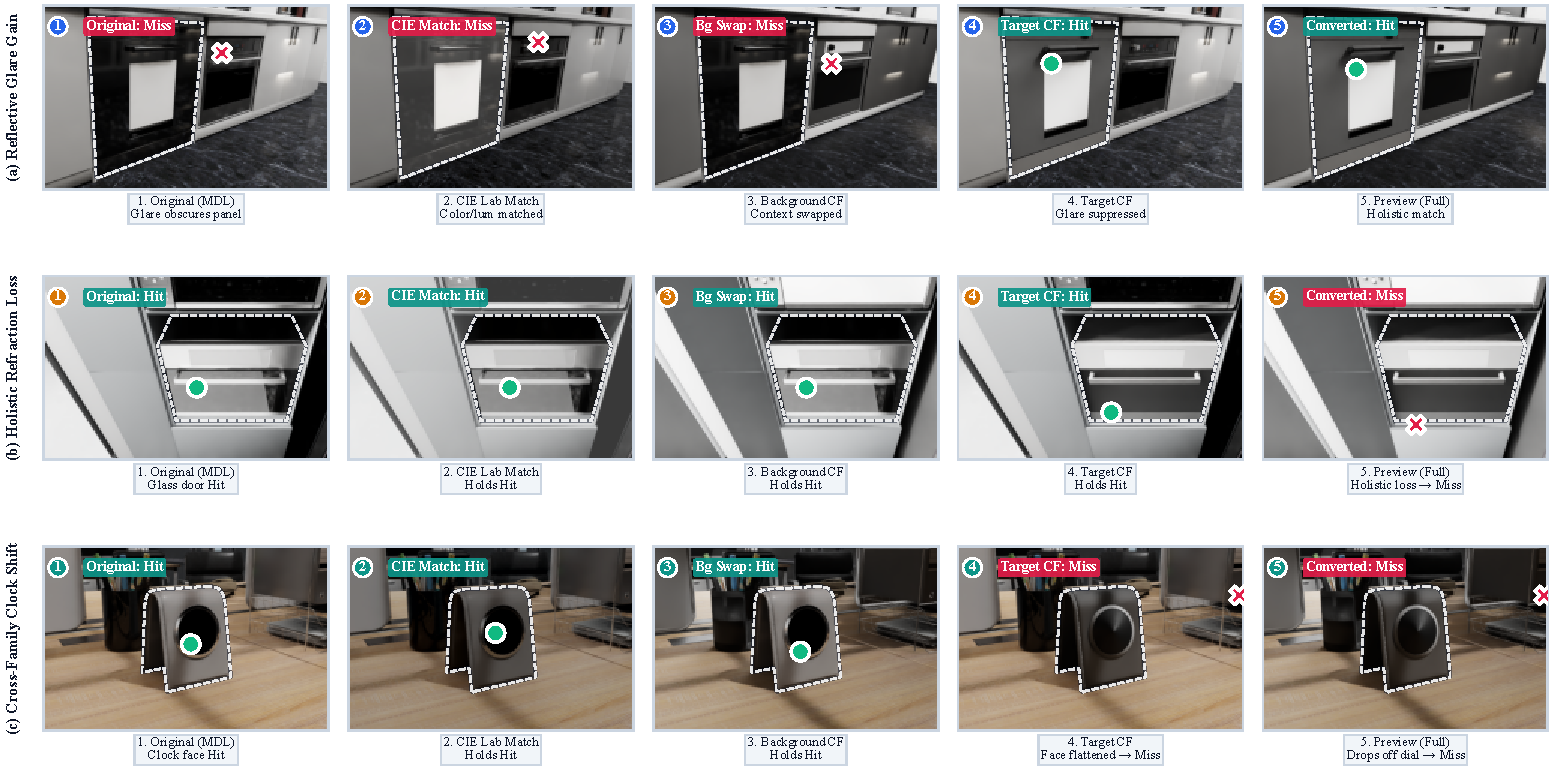
\includegraphics[width=\textwidth]{fig2_case_workflows.pdf}
\caption{\textbf{Representative optical mechanisms and five-condition counterfactual progressions (\textsc{Qwen3-VL-8B} and \textsc{InternVL3.5-8B-HF}).}
Each row traces one target through: (1)~\original\ (\textsc{MDL}) $I^O$, (2)~$\mathrm{CIE}~L^*a^*b^*$ photometric-matched control $I^{\text{photo}}$, (3)~background-only swap $I^B$, (4)~target-only swap $I^T$, and (5)~\converted\ (\texttt{UsdPreviewSurface}) $I^F$.
\emph{(a) Reflective Glare Gain (\textsc{Qwen3-VL-8B}):} glare removal inside the dishwasher silhouette ($I^T, I^F$) flips Miss $\to$ Hit whereas photometric recoloring alone fails ($I^{\text{photo}}$ Miss).
\emph{(b) Holistic Refraction Loss (\textsc{Qwen3-VL-8B}):} $I^O, I^{\text{photo}}, I^B$, and $I^T$ all retain Hit, whereas full scene conversion ($I^F$) flips Hit $\to$ Miss via a $2{\times}2$ scene--target interaction.
\emph{(c) Cross-Family Clock Shift (\textsc{InternVL3.5-8B-HF}):} target dial flattening in $I^T$ and $I^F$ shifts the predicted point off the arched desk clock (Hit $\to$ Miss).}
\label{fig:cases}
\end{figure*}

\paragraph{Thirty-scene benchmark and counterfactual pairs}
Our benchmark comprises \textbf{30 independent SimReady scenes} from \textsc{GRScenes} (20 residential and 10 commercial scenes), partitioned at the scene level prior to any feature fitting into \textbf{15 training (240 pairs), 5 validation (80 pairs), and 10 held-out test scenes (160 pairs)}. In each scene, eight distinct visible object instances are rendered from natural camera viewpoints at $1024 \times 768$ resolution, yielding \textbf{240 objects and 480 paired captures (960 images)}. Every target has a clear referring prompt (\texttt{"Point to the \dots"}) verified across both shader states and a pixel-exact segmentation mask $M_i^v \in \{0,1\}^{768 \times 1024}$ exported directly from the simulator. An automated mask-support check confirms zero empty masks and bit-identical target masks ($\mathrm{IoU} = 1.000$) in \textbf{473/480} pairs; the remaining 7 pairs exhibit subtle thin-rim anti-aliasing or alpha-cutout boundary shifts ($\mathrm{IoU} \ge 0.96$), tested explicitly via a dedicated sensitivity subset (Section~\ref{sec:mechanisms}). Three stratified control scenes (48 pairs, 96 images) provide three independent path-tracing re-renders each under fixed geometry and \original\ materials to quantify rendering variance. Figure~\ref{fig:cases} illustrates the five image conditions ($I^O, I^{\text{photo}}, I^B, I^T, I^F$) across three representative optical cases.

\begin{figure*}[!t]
\centering
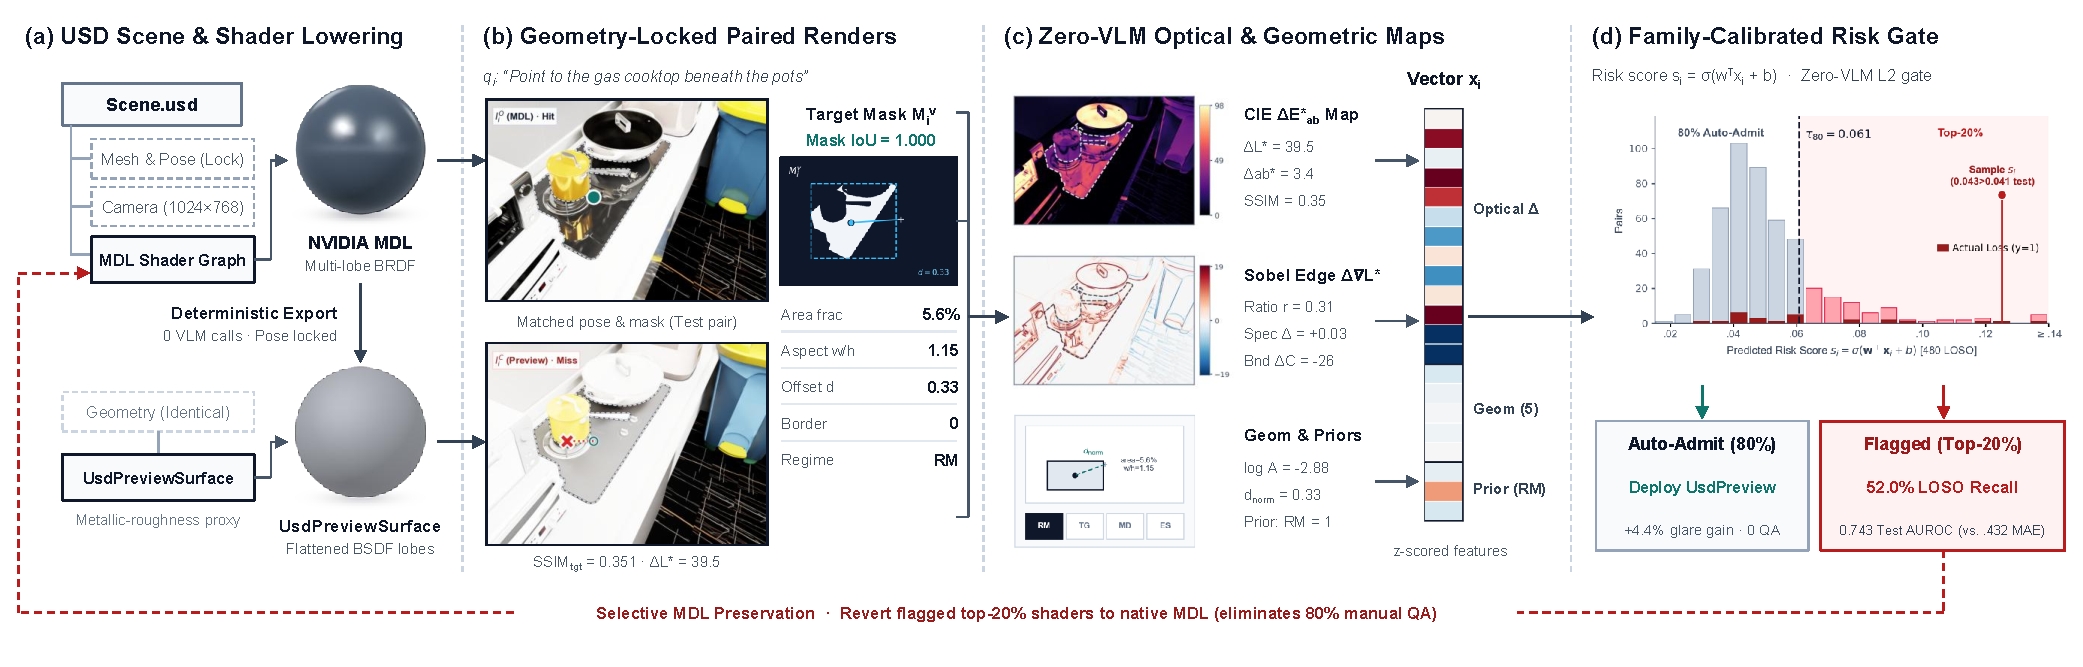
\includegraphics[width=\textwidth]{fig3_pipeline.pdf}
\caption{\textbf{End-to-end \textsc{ConvertAsset} shader-lowering and zero-\textsc{VLM} pre-deployment risk-gating pipeline.}
\emph{(a)} Deterministic \textsc{USD} export lowers multi-lobe \textsc{NVIDIA MDL} shading graphs into \texttt{UsdPreviewSurface} under locked meshes, poses, and camera extrinsics ($0$ \textsc{VLM} calls).
\emph{(b)} Geometry-locked paired renders $(I_i^O, I_i^C)$ and pixel-exact simulator masks $M_i^v$ expose directional localization regressions on held-out targets (here \textsc{Qwen3-VL-32B} flips Hit $\to$ Miss on a flattened reflective cooktop).
\emph{(c)} Zero-\textsc{VLM} perceptual ($\mathrm{CIE}~\Delta E_{ab}^*$), structural (\textsc{SSIM}, \textsc{Sobel} $\Delta\nabla L^*$), mask-geometry, and coarse regime-prior cues form a standardized feature vector $\mathbf{x}_i$.
\emph{(d)} A family-calibrated $\ell_2$ logistic gate scores regression risk $s_i = \sigma(\mathbf{w}^\top \mathbf{x}_i + b)$, auto-admitting $80\%$ of low-risk assets while routing the highest-risk $20\%$ back to selective \textsc{MDL} preservation ($52.0\%$ \textsc{LOSO} recall; $0.743$ test \textsc{AUROC} vs.\ $0.432$ global \textsc{RGB MAE}).}
\label{fig:pipeline}
\end{figure*}

\paragraph{Readout standardization, parser qualification, and paired estimands}
Because inconsistent coordinate conventions or non-deterministic sampling can masquerade as visual sensitivity (\ref{app:readout}), every evaluation executes unquantized \texttt{torch.bfloat16} inference (\texttt{device\_map="auto"}) with deterministic greedy decoding ($T{=}0$, \texttt{do\_sample=False}) under a uniform CUDA software environment, using a single canonical $0\text{--}1000$ normalized pointing prompt:
\begin{quote}\footnotesize\ttfamily
<query> Use normalized 0-1000 coordinates:\\
(0,0) top left, (1000,1000) bottom right.\\
Return exactly one line: Point: x, y
\end{quote}
To accommodate each family's native coordinate syntax without truncating bounding boxes or distorting predictions, every evaluated checkpoint first passes a 24-input pilot qualification gate ($\ge 90\%$ valid coordinate parses; Section~\ref{sec:grounding}, \ref{app:readout}), selecting one deterministic parser mode per family:
\begin{itemize}
    \item \texttt{strict}: exact \texttt{Point:\ x, y} format in $[0, 1000)$ (\textsc{Qwen3-VL-8B/32B}, \textsc{InternVL3.5-8B-HF}; $100\%$ pilot valid).
    \item \texttt{flex\_1000}: accepts \textsc{Qwen3-VL-2B}'s bare \texttt{(x, y)} tuples, JSON \texttt{point\_2d}, and 4-number box midpoints ($91.7\%$ pilot valid; $96.5\%$ full-benchmark valid).
    \item \texttt{molmo2\_1000}: extracts \textsc{Molmo2-8B}'s native \texttt{<points coords="1 1 x y">} and \texttt{<Point:\ x y>} tags ($100\%$ pilot valid; $99.1\%$ full valid).
    \item \texttt{unit\_float\_xy}: rescales \textsc{LLaVA-NeXT-Mistral-7B}'s unit-normalized $[0, 1]$ boxes and points to $0\text{--}1000$ midpoints ($100\%$ pilot valid; $99.2\%$ full valid).
\end{itemize}
For pair $i$ under condition $v \in \{O, C\}$, parsed coordinate $(u_i^v, v_i^v)$ maps to pixel $(u_i^v W / 1000,\, v_i^v H / 1000)$, defining binary grounding success $H_i^v = \mathbf{1}[(x_i^v, y_i^v) \in M_i^v]$. Beyond marginal hit rates $H^O$, $H^C$, and net delta $\Delta H = \mathbb{E}[H_i^C - H_i^O]$, we track paired decision-turnover rates:
\begin{align}
\mathrm{Loss} &= \Pr(H_i^O{=}1,\, H_i^C{=}0), \quad
\mathrm{Gain} = \Pr(H_i^O{=}0,\, H_i^C{=}1), \notag\\
\mathrm{Flip} &= \mathrm{Loss} + \mathrm{Gain},
\label{eq:turnover}
\end{align}
alongside conditional regression risk $\Pr(H_i^C{=}0 \mid H_i^O{=}1)$ and valid-pair Euclidean displacement $\Delta p_i = \|p_i^C - p_i^O\|_2$ in pixels. Because 16 camera pairs share each 3D environment, all confidence intervals and paired contrasts use \textbf{10,000-draw scene-cluster bootstrap resampling} over the $S=30$ scenes. Figure~\ref{fig:pipeline} illustrates the combined shader-lowering and zero-\textsc{VLM} risk-gating architecture.

\paragraph{Closed-loop navigation protocol (\textbf{RQ4})}
Section~\ref{sec:navigation} examines \textsc{InternNav/DualVLN} \citep{Wei2026Ground} over 99 paired unseen episodes across three KuJiaLe \texttt{val\_unseen} apartments (33 episodes per scene, 198 rollouts) sharing identical language instructions, starting poses, and step budgets.

\section{Variance Floor, Scaling Laws, and Four-Family Generalization (\textbf{RQ1})}
\label{sec:grounding}

\subsection{Four-Level Variance Decomposition Across Six Checkpoints}
\label{sec:variance}

Before attributing localization shifts to surface material conversion, one must establish how much variance stems from inference repeatability, decoding stochasticity, or Monte Carlo path tracing \citep{Zhao2021Calibrate}. On three stratified control scenes (48 paired captures, 96 images), Table~\ref{tab:variance} and Figure~\ref{fig:variance_scaling}(a) decompose four nested variability levels across all six checkpoints:
\begin{enumerate}
    \item \textbf{Level 1 (Greedy process repeat: $0.00\%$, $0.00\,\mathrm{px}$ on all six checkpoints).} Across repeated deterministic inference runs ($T{=}0$, \texttt{do\_sample=False})---three runs on \textsc{Qwen3-VL-8B} and \textsc{Qwen3-VL-32B} (288 pairwise comparisons each) and two runs on \textsc{Qwen3-VL-2B}, \textsc{InternVL3.5-8B-HF}, \textsc{Molmo2-8B}, and \textsc{LLaVA-NeXT-Mistral-7B} (96 comparisons each)---pairwise hit disagreement and spatial coordinate displacement remain strictly zero ($0.00\%$, $0.00\,\mathrm{px}$).
    \item \textbf{Level 2 (Stochastic decoding noise: $8.96\%$ pairwise, $16.67\%$ any-flip).} Repeating the same 96 frozen images across five stochastic draws ($T{=}0.2$, $\text{top-}p{=}0.95$) on \textsc{Qwen3-VL-8B} (960 pairwise checks) produces $94.38\%$ response phrasing variation, $8.96\%$ pairwise hit disagreement, $16.67\%$ of inputs with at least one pass/fail flip, and $16.37\,\mathrm{px}$ mean displacement. This stochastic noise floor explains why stochastic sampling confounds shading studies (\ref{app:archive}) and motivates locking greedy $T{=}0$ decoding to isolate visual sensitivity.
    \item \textbf{Level 3 (Monte Carlo ray-tracing re-render floor).} Holding geometry, cameras, prompts, and \original\ materials fixed across three independent path-tracing renders (96 pairs per model) yields $7.29\%$ ($7/96$, $30.96\,\mathrm{px}$) flips on \textsc{Qwen3-VL-2B}, $5.21\%$ ($5/96$, $24.38\,\mathrm{px}$) on \textsc{LLaVA-NeXT-Mistral-7B}, $3.13\%$ ($3/96$, $9.52\,\mathrm{px}$) on \textsc{Qwen3-VL-8B}, $1.04\%$ ($1/96$) on both \textsc{InternVL3.5-8B-HF} ($10.38\,\mathrm{px}$) and \textsc{Qwen3-VL-32B} ($6.39\,\mathrm{px}$), and $0.00\%$ ($0/96$, $5.98\,\mathrm{px}$) on \textsc{Molmo2-8B}.
    \item \textbf{Level 4 (Material conversion on the same 48 control pairs).} Lowering \textsc{MDL} to \usdps{} induces \textbf{$2.00\times$ to $6.00\times$} the flip rate of independent path-tracing repeats ($20.83\%$ on 2B [$2.86\times$], $10.42\%$ on \textsc{LLaVA-NeXT} [$2.00\times$], $8.33\%$ on 8B [$2.67\times$], $6.25\%$ on \textsc{InternVL3.5-8B} [$6.00\times$], $4.17\%$ on \textsc{32B} [$4.00\times$], and $4.17\%$ vs.\ $0.00\%$ [$>4\times$] on \textsc{Molmo2-8B}), alongside $2.1\times$ to $7.0\times$ larger spatial shifts ($23.26\text{--}65.64\,\mathrm{px}$).
\end{enumerate}

\begin{table*}[!t]
\centering\scriptsize
\resizebox{\textwidth}{!}{% Verified from paper/shared/evidence/raw/cviu_v3/variance_decomposition.json
\begin{tabular*}{\textwidth}{@{\extracolsep{\fill}}llrrrrrr@{}}
\toprule
Model (Strict \texttt{bfloat16}) & Family & L1 Greedy & \multicolumn{2}{c}{L3: Re-Render Floor (96)} & \multicolumn{2}{c}{L4: Conversion (48 pairs)} & L4 / L3 \\
\cmidrule(lr){4-5} \cmidrule(lr){6-7}
 & & Disagr.\ (pairs) & Flip Rate & Shift (px) & Flip Rate & Shift (px) & Ratio \\
\midrule
Qwen3-VL-2B & Qwen3-VL & 0.00\% (96) & 7.29\% (7/96) & 30.96 & \textbf{20.83\%} (10/48) & \textbf{65.64} & 2.86$\times$ \\
LLaVA-NeXT-Mistral-7B & Mistral + CLIP & 0.00\% (96) & 5.21\% (5/96) & 24.38 & \textbf{10.42\%} (5/48) & \textbf{59.90} & 2.00$\times$ \\
InternVL3.5-8B-HF & InternVL3.5 & 0.00\% (96) & 1.04\% (1/96) & 10.38 & \textbf{6.25\%} (3/48) & \textbf{39.23} & 6.00$\times$ \\
Qwen3-VL-8B & Qwen3-VL & 0.00\% (288) & 3.13\% (3/96) & 9.52 & \textbf{8.33\%} (4/48) & \textbf{23.83} & 2.67$\times$ \\
Molmo2-8B & Molmo2 (SigLIP-2) & 0.00\% (96) & 0.00\% (0/96) & 5.98 & \textbf{4.17\%} (2/48) & \textbf{41.64} & $>4\times$ \\
Qwen3-VL-32B & Qwen3-VL & 0.00\% (288) & 1.04\% (1/96) & 6.39 & \textbf{4.17\%} (2/48) & \textbf{23.26} & 4.00$\times$ \\
\midrule
\multicolumn{8}{@{}l}{\emph{Level 2 stochastic decoding baseline (Qwen3-VL-8B, $T{=}0.2$, $\text{top-}p{=}0.95$, 5 draws on same 96 frozen images, 960 pairs):}} \\
\multicolumn{2}{@{}l}{Pairwise hit disagreement / any-flip across 5 draws} & \multicolumn{6}{r@{}}{8.96\% pairwise disagreement (16.67\% inputs with $\ge 1$ flip; 94.38\% text change; 16.37\,px shift)} \\
\bottomrule
\end{tabular*}
}
\caption{Four-level variance decomposition over the three stratified control scenes (48 object pairs, 96 images) across all six checkpoints. Greedy decoding eliminates sampling stochasticity ($0.00\%$ everywhere), establishing material conversion well above the independent ray-tracing noise floor.}
\label{tab:variance}
\end{table*}

\begin{figure*}[!t]
\centering
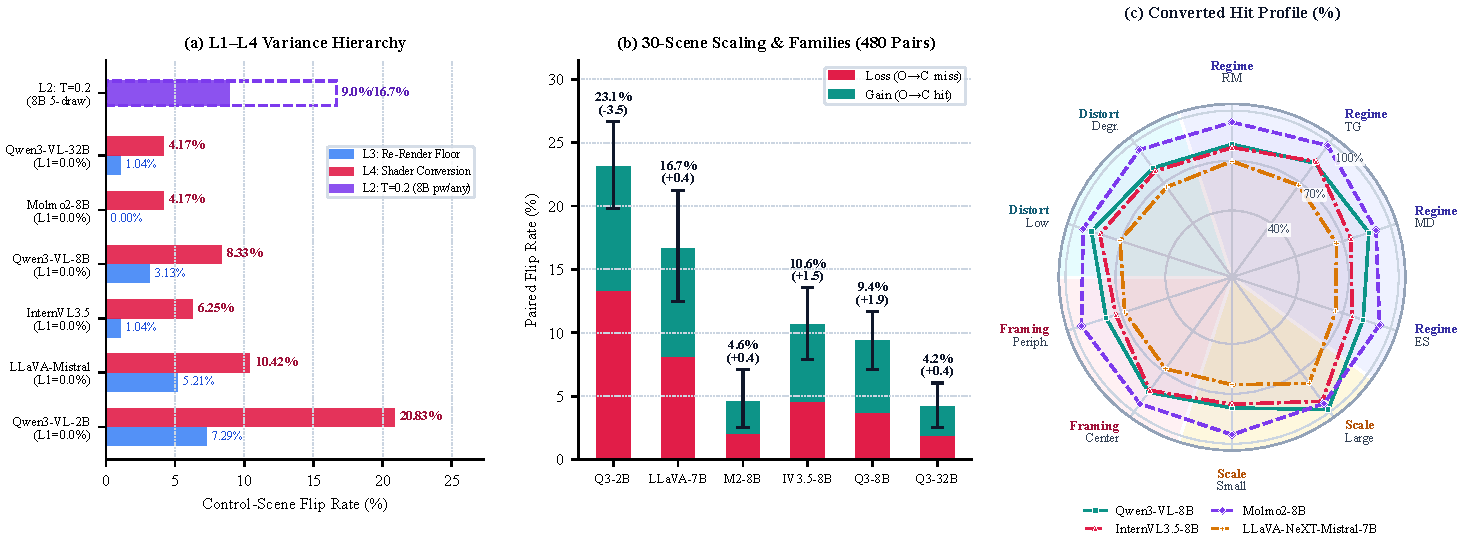
\includegraphics[width=\textwidth]{fig4_variance_and_polar.pdf}
\caption{\textbf{Four-level variance hierarchy, 30-scene scaling across four families, and converted hit profile.}
\emph{(a)} Across all six checkpoints, greedy $T{=}0$ inference eliminates decoding noise ($0.00\%$), while \textsc{MDL} $\to$ \usdps{} conversion (Level 4) induces $2.0\times$ to $6.0\times$ more flips than same-material ray-tracing repeats (Level 3; $4.17\%$ vs.\ $0.00\%$ on \textsc{Molmo2-8B}).
\emph{(b)} Across 30 scenes (480 pairs), scaling \textsc{Qwen3-VL} $16\times$ (2B $\to$ 8B $\to$ 32B) reduces turnover from $23.13\%$ to $4.17\%$, yet bidirectional swaps persist across all four independent families (\textsc{InternVL3.5}, \textsc{Molmo2}, \textsc{LLaVA-NeXT-Mistral}). Error bars denote 10,000-draw scene-cluster 95\% CIs.
\emph{(c)} Multi-axis polar profile of \converted\ hit rate ($H_C$, \%) across residential/commercial domains, optical regimes, and target scales.}
\label{fig:variance_scaling}
\end{figure*}

\subsection{30-Scene Scaling Laws and Four-Family Generalization}
\label{sec:scaling}

Table~\ref{tab:grounding_v3} and Figure~\ref{fig:variance_scaling}(b)--(c) evaluate all six checkpoints across the full 30-scene suite (480 paired captures, $96.5\%\text{--}100.0\%$ valid parse rates). Four empirical patterns characterize how shader lowering affects grounding behavior:

\paragraph{1.\ Near-zero net deltas conceal $4.17\%\text{--}23.13\%$ bidirectional turnover.}
Three checkpoints spanning completely distinct model families record the exact same aggregate delta of $+0.42\%$ between \original\ and \converted: \textsc{LLaVA-NeXT-Mistral-7B} ($67.50\% \to 67.92\%$, 95\% CI $[-3.33\%, +3.96\%]$), \textsc{Qwen3-VL-32B} ($91.67\% \to 92.08\%$, CI $[-1.25\%, +2.29\%]$), and \textsc{Molmo2-8B} ($93.96\% \to 94.38\%$, CI $[-1.67\%, +2.50\%]$). Underneath those nearly flat averages, \textsc{LLaVA-NeXT-Mistral-7B} reverses outcomes on $16.67\%$ of objects ($8.13\%$ Loss, $8.54\%$ Gain; $65.08\,\mathrm{px}$ mean displacement), \textsc{Molmo2-8B} flips $4.58\%$ ($2.08\%$ Loss, $2.50\%$ Gain; $33.80\,\mathrm{px}$), and \textsc{Qwen3-VL-32B} flips $4.17\%$ ($1.88\%$ Loss, $2.29\%$ Gain; $20.78\,\mathrm{px}$). Smaller models exhibit even larger turnover behind modest marginal changes: \textsc{Qwen3-VL-2B} declines $-3.54\%$ net ($66.67\% \to 63.13\%$) while flipping \textbf{$23.13\%$} of pairs ($13.33\%$ Loss, $9.79\%$ Gain; $69.70\,\mathrm{px}$).

\paragraph{2.\ Scaling $16\times$ dampens turnover monotonically yet leaves an irreducible floor}
Within the \textsc{Qwen3-VL} family \citep{Bai2025Qwen3}, scaling from 2B $\to$ 8B $\to$ 32B lifts baseline \original\ accuracy ($66.67\% \to 81.25\% \to 91.67\%$), reduces conditional regression risk $\Pr(H^C{=}0 \mid H^O{=}1)$ roughly tenfold ($20.00\% \to 4.62\% \to 2.05\%$), and lowers overall decision turnover from $23.13\%$ to $9.38\%$ and $4.17\%$ (paired scene-cluster reduction $-18.96$ pp from 2B to 32B, 95\% CI $[-22.92, -15.00]$; $-5.21$ pp from 8B to 32B, CI $[-7.71, -2.71]$). Even at 32B, however, turnover ($4.17\%$) stays $4\times$ above its ray-tracing repeat floor ($1.04\%$) with $20.78\,\mathrm{px}$ average point displacement, while conditional recovery on initially missed objects remains nearly constant around $28\%\text{--}30\%$ across all three scales ($29.38\%$ at 2B, $30.00\%$ at 8B, $27.50\%$ at 32B).

\paragraph{3.\ Cross-family invariance and architecture-specific failures ($85.7\%$ divergence)}
Extending evaluation to three additional VLM families at the 7B--8B scale shows that shader sensitivity generalizes across backbones:
\begin{itemize}
    \item \textsc{InternVL3.5-8B-HF} \citep{Wang2025InternVL35} tracks \textsc{Qwen3-VL-8B} closely in hit rate ($78.54\% \to 80.00\%$, $\Delta H = +1.46\%$) and decision turnover ($10.63\%$; paired difference $+1.25\%$ vs.\ \textsc{Qwen3-VL-8B}, CI $[-2.29\%, +4.79\%]$), though with larger spatial displacements ($47.11\,\mathrm{px}$ vs.\ $27.23\,\mathrm{px}$, paired $+19.88\,\mathrm{px}$).
    \item \textsc{Molmo2-8B} \citep{Clark2026Molmo2}, a \textsc{SigLIP-2} pointing specialist, attains the highest accuracy ($93.96\% \to 94.38\%$) and lowest 8B turnover ($4.58\%$, $-4.79\%$ vs.\ \textsc{Qwen3-VL-8B}, CI $[-7.08\%, -2.50\%]$, with $41.38\%$ conditional recovery), yet its conversion flip rate remains well above its zero ray-tracing noise floor ($4.17\%$ vs.\ $0.00\%$ on controls; $33.80\,\mathrm{px}$ displacement).
    \item \textsc{LLaVA-NeXT-Mistral-7B} \citep{Liu2024LLaVANeXT}, pairing a \textsc{Mistral-7B} language backbone with a \textsc{CLIP} vision encoder, scores $67.50\% \to 67.92\%$ ($\Delta H = +0.42\%$) while incurring $16.67\%$ bidirectional turnover ($+7.29\%$ vs.\ \textsc{Qwen3-VL-8B}, CI $[+3.33\%, +11.67\%]$; $65.08\,\mathrm{px}$ shift).
\end{itemize}
Comparing the four $\ge$7B architectures (\textsc{Qwen3-VL-8B}, \textsc{InternVL3.5-8B-HF}, \textsc{Molmo2-8B}, and \textsc{LLaVA-NeXT-Mistral-7B}) across all 480 pairs reveals that $77$ pairs undergo at least one regression (\emph{Loss}), yet \textbf{$66/77$ ($85.7\%$)} fail on only one architecture (10 pairs regress on two families, 1 pair on three, and none on all four). Specialization improves baseline robustness without removing material vulnerability, and largely disjoint targets fail across different vision-language backbones---a divergence that directly shapes pre-deployment risk gating in Section~\ref{sec:risk_gate}.

\begin{table*}[!t]
\centering\scriptsize
\resizebox{\textwidth}{!}{% Verified from paper/shared/evidence/raw/cviu_v3/scaling_and_families.json (30 scenes, 480 pairs)
\begin{tabular}{@{}lllrrrrrr@{}}
\toprule
Model & Family (Backbone) & Parser (Val.\ \%) & $H_O$ (\%) & $H_C$ (\%) & $\Delta H$ [95\% CI] & Flip (\%) [95\% CI] & Loss / Gain & Shift (px) \\
\midrule
Qwen3-VL-2B & Qwen3-VL (2B) & \texttt{flex\_1000} (96.5) & 66.67 & 63.13 & -3.54 [-8.33, +1.25] & 23.13 [19.79, 26.67] & 13.33 / 9.79 & 69.70 \\
LLaVA-NeXT-Mistral-7B & Mistral-7B + CLIP & \texttt{unit\_float\_xy} (99.2) & 67.50 & 67.92 & +0.42 [-3.33, +3.96] & 16.67 [12.50, 21.25] & 8.13 / 8.54 & 65.08 \\
InternVL3.5-8B-HF & InternVL3.5 (8B) & \texttt{strict} (100.0) & 78.54 & 80.00 & +1.46 [-0.42, +3.33] & 10.63 [7.92, 13.54] & 4.58 / 6.04 & 47.11 \\
Qwen3-VL-8B & Qwen3-VL (8B) & \texttt{strict} (99.5) & 81.25 & 83.13 & +1.88 [-0.42, +4.17] & 9.38 [7.08, 11.67] & 3.75 / 5.63 & 27.23 \\
Molmo2-8B & SigLIP-2 + Qwen3-8B & \texttt{molmo2\_1000} (99.1) & 93.96 & 94.38 & +0.42 [-1.67, +2.50] & 4.58 [2.50, 7.08] & 2.08 / 2.50 & 33.80 \\
Qwen3-VL-32B & Qwen3-VL (32B) & \texttt{strict} (99.8) & 91.67 & 92.08 & +0.42 [-1.25, +2.29] & 4.17 [2.50, 6.04] & 1.88 / 2.29 & 20.78 \\
\midrule
\multicolumn{5}{@{}l}{Paired scaling contrast: Qwen3-VL-32B minus 2B / 8B (Flip diff.)} & & \textbf{-18.96} / \textbf{-5.21} & \multicolumn{2}{r@{}}{[-22.92, -15.00] / [-7.71, -2.71]} \\
\multicolumn{5}{@{}l}{Cross-family vs.\ Qwen3-VL-8B: InternVL3.5 / Molmo2 / LLaVA-Mistral} & & +1.25 / -4.79 / +7.29 & \multicolumn{2}{r@{}}{[-2.29,+4.79] / [-7.08,-2.50] / [+3.33,+11.67]} \\
\multicolumn{9}{@{}l}{\emph{Architecture overlap across 4 $\ge$7B families:} 77/480 pairs lose on $\ge 1$ family, with \textbf{66/77 (85.7\%)} unique to a single architecture (10 in 2, 1 in 3, 0 in 4).} \\
\bottomrule
\end{tabular}
}
\caption{Full 30-scene (480-pair) visual grounding results across four VLM families and six checkpoints under deterministic greedy decoding ($T{=}0$), with paired 10,000-draw scene-cluster 95\% confidence intervals. Near-zero net accuracy shifts ($\Delta H$) conceal substantial bidirectional Loss/Gain turnover and $85.7\%$ single-architecture regression divergence.}
\label{tab:grounding_v3}
\end{table*}

\section{Causal Optical Mechanisms and Pre-Deployment Risk Gating (\textbf{RQ2} \& \textbf{RQ3})}
\label{sec:mechanisms}

Having established that shader-induced turnover persists across model scales and four distinct architectures well above path-tracing noise, we next investigate its optical causes (\textbf{RQ2}) and ask whether regressions can be anticipated automatically before invoking any VLM (\textbf{RQ3}).

\subsection{2,880 Cross-Family Silhouette Counterfactuals and Photometric Controls}
\label{sec:counterfactuals}

Explaining material sensitivity from natural conversion pairs alone faces two confounds: foreground--background edits over rectangular boxes mix surrounding context inside the box, and simple shifts in object brightness or color can change visual salience \citep{Burgert2025NotTexture} independently of higher-order shader properties. To isolate these optical channels without introducing fresh path-tracing noise, we construct \textbf{three pixel-exact counterfactuals} for every pair (1,440 images) from the frozen renders and simulator segmentation masks $M_i^v$, evaluating all conditions on \emph{two independent 8B architectures} (\textsc{Qwen3-VL-8B} and \textsc{InternVL3.5-8B-HF}; \textbf{2,880 evaluations total}):
\begin{enumerate}
    \item \textbf{Target-only shader conversion ($I_i^T$):} Pixels inside the converted target mask $M_i^C$ take \converted\ values while the background remains \original, using symmetric boundary compositing where mask edges differ in 7/480 pairs.
    \item \textbf{Background-only shader conversion ($I_i^B$):} Pixels inside $M_i^O$ remain \original\ while surrounding scene context takes \converted\ values.
    \item \textbf{Photometric-matched control ($I_i^{\text{photo}}$):} Starting from $I_i^O$, affine channel matching in $\mathrm{CIE}~L^*a^*b^*$ aligns target and background color and luminance means and standard deviations separately to $I_i^C$, while preserving native \textsc{MDL} textures, specular reflections, and high-frequency detail.
\end{enumerate}

\begin{table*}[!t]
\centering\scriptsize
\resizebox{\textwidth}{!}{% Verified from paper/shared/evidence/raw/cviu_v3/optical_mechanisms.json (2,880 counterfactual evaluations)
\begin{tabular}{@{}lrrrrrrrrrrr@{}}
\toprule
Condition / Optical Stratum & $N$ & \multicolumn{5}{c}{Qwen3-VL-8B (1,440 CF evals)} & \multicolumn{5}{c}{InternVL3.5-8B-HF (1,440 CF evals)} \\
\cmidrule(lr){3-7} \cmidrule(lr){8-12}
 & & $H$ (\%) & Flip [95\% CI] & L / G (\%) & Shift & Net $\Delta$ & $H$ (\%) & Flip [95\% CI] & L / G (\%) & Shift & Net $\Delta$ \\
\midrule
\multicolumn{12}{@{}l}{\emph{Panel A: 480-pair natural counterfactual decomposition (2,880 synthesized CF evaluations across 2 independent 8B families)}} \\
Original (\textsc{MDL}) $I^O$ & 480 & 81.25 & --- & --- & --- & --- & 78.54 & --- & --- & --- & --- \\
Photometric ($\mathrm{CIE}~L^*a^*b^*$) $I^{\text{photo}}$ & 480 & 80.83 & 5.83 [3.75, 8.13] & 3.13 / 2.71 & 20.27 & -0.42 & 79.38 & 7.08 [5.00, 9.38] & 3.13 / 3.96 & 32.26 & +0.83 \\
Background-converted only $I^B$ & 480 & 80.63 & 6.46 [4.58, 8.54] & 3.54 / 2.92 & 23.37 & -0.63 & 80.21 & 9.17 [6.67, 11.88] & 3.75 / 5.42 & 38.97 & +1.67 \\
Target-converted only $I^T$ & 480 & 80.63 & 8.13 [5.63, 10.83] & 4.38 / 3.75 & 24.16 & -0.63 & 81.25 & 9.79 [7.29, 12.50] & 3.54 / 6.25 & 37.47 & +2.71 \\
Full converted (\texttt{Preview}) $I^F$ & 480 & 83.13 & \textbf{9.38} [7.08, 11.67] & 3.75 / 5.63 & 27.23 & +1.88 & 80.00 & \textbf{10.63} [7.92, 13.54] & 4.58 / 6.04 & 47.11 & +1.46 \\
\midrule
Non-photometric residual ($I^F - I^{\text{photo}}$, 480) & 480 & +2.29 & \textbf{+3.54} [+1.25, +5.83] & +0.63 / +2.92 & +6.96 & --- & +0.63 & \textbf{+3.54} [+1.04, +6.04] & +1.46 / +2.08 & +14.85 & --- \\
Non-photometric residual (473 id.-mask) & 473 & +2.11 & \textbf{+3.38} [+1.26, +5.70] & +0.63 / +2.75 & +6.98 & --- & +0.42 & \textbf{+3.38} [+0.84, +5.97] & +1.48 / +1.90 & +14.79 & --- \\
\midrule
\multicolumn{12}{@{}l}{\emph{Panel B: Paired stratification of Full ($I^F$) vs.\ Original ($I^O$) by prior surface optical regime}} \\
Reflective / Metallic & 158 & 79.75 & 10.76 & 3.16 / 7.59 & --- & \textbf{+4.43} & 77.85 & 10.76 & 5.06 / 5.70 & --- & +0.63 \\
Transparent / Glass & 176 & 84.66 & 9.66 & 4.55 / 5.11 & --- & +0.57 & 85.80 & 9.66 & 3.98 / 5.68 & --- & +1.70 \\
Matte / Diffuse & 88 & 86.36 & 10.23 & 4.55 / 5.68 & --- & +1.14 & 75.00 & 10.23 & 5.68 / 4.55 & --- & \textbf{-1.14} \\
Emissive / Screen & 58 & 82.76 & 3.45 & 1.72 / 1.72 & --- & +0.00 & 75.86 & 13.79 & 3.45 / 10.34 & --- & \textbf{+6.90} \\
\bottomrule
\end{tabular}
}
\caption{Cross-family causal optical decomposition on \textsc{Qwen3-VL-8B} and \textsc{InternVL3.5-8B-HF} over all 480 natural pairs (2,880 total counterfactual inferences), sensitivity check on 473 bit-identical mask pairs, and stratification by prior surface optical category.}
\label{tab:mechanisms_v3}
\end{table*}

\begin{figure*}[!t]
\centering
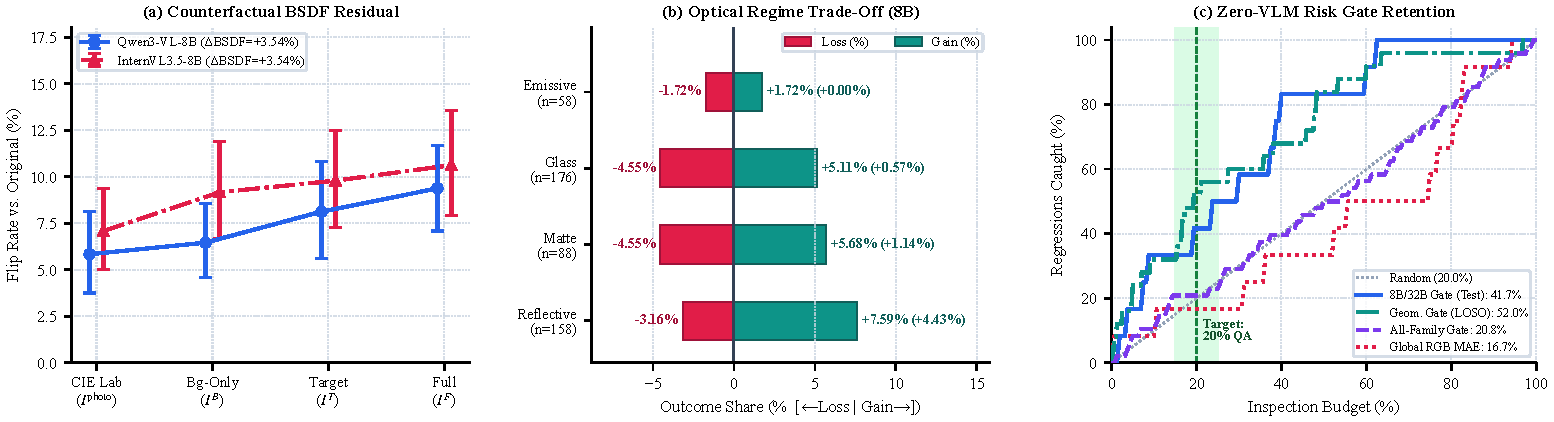
\includegraphics[width=\textwidth]{fig5_causal_and_risk.pdf}
\caption{\textbf{Cross-family optical mechanism decomposition and zero-\textsc{VLM} pre-deployment risk gating (\textbf{RQ2} \& \textbf{RQ3}).}
\emph{(a)} Across 2,880 counterfactual evaluations on \textsc{Qwen3-VL-8B} and \textsc{InternVL3.5-8B-HF}, matched $\mathrm{CIE}~L^*a^*b^*$ luminance/color salience ($I^{\text{photo}}$) leaves an identical \textbf{$+3.54\%$} non-photometric \textsc{BSDF} flip residual ($I^F - I^{\text{photo}}$) on both independent families.
\emph{(b)} Surface optical regimes explain mean-delta cancellation on \textsc{Qwen3-VL-8B}: \emph{Reflective/Metallic} targets gain $+4.43\%$ via glare suppression ($7.59\%$ Gain vs.\ $3.16\%$ Loss), whereas \emph{Transparent/Glass} and \emph{Matte/Diffuse} trade regressions against improvements.
\emph{(c)} Zero-\textsc{VLM} selective quality-assurance curves: routing the highest-risk $20\%$ of pairs captures $41.7\%$ of held-out \textsc{Qwen3-VL} regressions ($52.0\%$ in 30-scene \textsc{LOSO}) vs.\ $16.7\%$ for global \textsc{RGB MAE}, whereas pooling heterogeneous architectures (\texttt{Any-Family}) lowers \textsc{AUROC} ($0.582$ test) because $85.7\%$ of regressions are model-specific.}
\label{fig:mechanisms}
\label{fig:risk_gate}
\end{figure*}

Table~\ref{tab:mechanisms_v3} and Figure~\ref{fig:mechanisms}(a)--(b) yield three consistent optical findings across families:
\begin{itemize}
    \item \textbf{Both 8B architectures exhibit an identical $+3.54\%$ non-photometric BSDF residual.} On \textsc{Qwen3-VL-8B}, matching per-region $\mathrm{CIE}~L^*a^*b^*$ luminance and chromatic moments alone ($I^{\text{photo}}$) accounts for $5.83\%$ flips ($20.27\,\mathrm{px}$ shift; $80.83\%$ hit rate), compared with $9.38\%$ under full shader conversion ($I^F$, $27.23\,\mathrm{px}$), leaving a significant non-photometric residual of \textbf{$+3.54\%$ (95\% CI $[+1.25\%, +5.83\%]$)}. \textsc{InternVL3.5-8B-HF} displays the exact same residual: $I^{\text{photo}}$ induces $7.08\%$ flips ($32.26\,\mathrm{px}$) versus $10.63\%$ under $I^F$ ($47.11\,\mathrm{px}$), again leaving \textbf{$+3.54\%$ (95\% CI $[+1.04\%, +6.04\%]$)}. Restricting to the $473/480$ pairs with bit-identical simulator masks ($\mathrm{IoU}=1.0$) produces virtually unchanged residuals of $+3.38\%$ on both models ($[+1.26\%, +5.70\%]$ on \textsc{Qwen3-VL-8B}; $[+0.84\%, +5.97\%]$ on \textsc{InternVL3.5-8B-HF}).
    \item \textbf{Target dominance and backbone-dependent context coupling.} Both families flip more frequently under target-only shader conversion ($I^T$: $8.13\%$ on \textsc{Qwen3-VL-8B}, $9.79\%$ on \textsc{InternVL3.5-8B-HF}) than background-only conversion ($I^B$: $6.46\%$ and $9.17\%$; paired $T{-}B$ $+1.67\%$ CI $[-0.42\%, +3.96\%]$ and $+0.63\%$ CI $[-1.88\%, +2.92\%]$). Their $2\times 2$ interaction ($I^F - I^T - I^B + I^O$) diverges across models: on \textsc{Qwen3-VL-8B}, isolated target or context swaps modestly reduce accuracy ($81.25\% \to 80.63\%$) before full scene conversion restores illumination coherence ($83.13\%$, interaction $+3.13\%$, CI $[0.00\%, +6.25\%]$), whereas \textsc{InternVL3.5-8B-HF} gains under partial swaps ($80.21\%\text{--}81.25\%$) and settles at $80.00\%$ (interaction $-2.92\%$, CI $[-6.46\%, +0.42\%]$).
    \item \textbf{Optical regime trade-offs behind near-zero aggregate shifts.} Stratifying all 480 pairs by prior surface class (Table~\ref{tab:mechanisms_v3}, Panel~B; Figure~\ref{fig:mechanisms}(b)) reveals the opposing mechanisms that cancel in global averages. On \textsc{Qwen3-VL-8B}, \emph{Reflective/Metallic} targets ($n{=}158$, e.g., stainless appliances and chrome fixtures) improve by $+4.43\%$ ($75.32\% \to 79.75\%$, $7.59\%$ Gain vs.\ $3.16\%$ Loss) as distracting glare recedes, whereas \emph{Transparent/Glass} ($n{=}176$, $+0.57\%$) and \emph{Matte/Diffuse} ($n{=}88$, $+1.14\%$) trade losses against gains; pixel-distortion grouping confirms that \emph{Low-Distortion} captures ($n{=}133$) gain $+3.76\%$ ($84.96\% \to 88.72\%$) while heavily \emph{Specular-Stripped} targets ($n{=}14$) decline $-7.14\%$ ($85.71\% \to 78.57\%$). By contrast, \textsc{InternVL3.5-8B-HF} shows its largest gain on \emph{Emissive/Screen} targets ($n{=}58$, $+6.90\%$, $68.97\% \to 75.86\%$) and a net $-1.14\%$ drop on \emph{Matte/Diffuse} surfaces ($76.14\% \to 75.00\%$).
\end{itemize}

\subsection{Zero-\textsc{VLM} Pre-Deployment Conversion Risk Gate (\textbf{RQ3})}
\label{sec:risk_gate}

Because improvements and regressions stem from distinct optical mechanisms, generic image-difference scores such as global \textsc{RGB MAE} cannot reliably identify hazardous shader exports. We examine whether an automated risk auditor requiring zero \textsc{VLM} inference during export can flag conversion regressions in advance, and how architectural divergence alters gating effectiveness.

For each capture pair, we compute 21 automated cues (\texttt{deploy\_auto}; full inventory in~\ref{app:mechanisms_risk}): five simulator mask-geometry attributes ($\log_{10}$ area fraction, bounding-box aspect ratio, normalized distance from frame center, border-touch indicator, and mask $\mathrm{IoU}$), thirteen paired optical, chromatic, and structural deltas (global/target/background \textsc{RGB MAE}, target lightness and chromatic shifts in $\mathrm{CIE}~L^*a^*b^*$, target lightness-std ratio, target/background \textsc{SSIM}, target Sobel edge ratio, target/ring specular-fraction shifts, and inner/outer contour contrast shifts), and three coarse target-category priors (transparent/glass, reflective appliance/metal, emissive/screen). We fit standardized $\ell_2$-regularized logistic regression on the 15 training scenes ($n{=}240$), select regularization $C$ on the 5 validation scenes ($n{=}80$), and evaluate on the 10 held-out test scenes ($n{=}160$) as well as 30-scene Leave-One-Scene-Out (\textsc{LOSO}) cross-validation across all 480 pairs.

\begin{table*}[!t]
\centering\scriptsize
\resizebox{\textwidth}{!}{% Verified from paper/shared/evidence/raw/cviu_v3/risk_auditor.json
\begin{tabular}{@{}llrrrrrr@{}}
\toprule
Target Regressions & Zero-VLM Predictor / Feature Set & \multicolumn{3}{c}{Held-Out Test (10 scenes, $n{=}160$)} & \multicolumn{3}{c}{30-Scene LOSO ($n{=}480$)} \\
\cmidrule(lr){3-5} \cmidrule(lr){6-8}
 & & AUROC & AUPRC & R@20\% & AUROC & AUPRC & R@20\% \\
\midrule
\multirow{6}{*}{Any 8B/32B Loss (\textsc{Qwen3-VL})} & \texttt{deploy\_auto} (21 automated features) & \textbf{0.743} & 0.195 & 0.417 & 0.653 & 0.137 & 0.360 \\
 & \texttt{geometry\_only} (5 mask features) & 0.742 & \textbf{0.216} & 0.417 & \textbf{0.732} & \textbf{0.184} & \textbf{0.520} \\
 & \texttt{pixel\_only} (13 appearance deltas) & 0.606 & 0.130 & 0.333 & 0.502 & 0.102 & 0.320 \\
 & \texttt{all\_with\_review\_priors} (24 features) & 0.713 & 0.171 & 0.417 & 0.644 & 0.127 & 0.320 \\
 & \texttt{baseline\_target\_rgb\_mae} & 0.557 & 0.172 & 0.417 & 0.577 & 0.140 & 0.280 \\
 & \texttt{baseline\_global\_rgb\_mae} & 0.432 & 0.150 & 0.167 & 0.490 & 0.090 & 0.240 \\
\midrule
\multirow{2}{*}{Qwen3-VL-8B Loss} & \texttt{deploy\_auto} / \texttt{geometry\_only} & 0.632 / 0.650 & 0.080 / 0.092 & 0.286 / 0.143 & 0.594 / 0.666 & 0.077 / 0.096 & 0.389 / 0.389 \\
 & \texttt{baseline\_global\_rgb\_mae} & 0.413 & 0.177 & 0.143 & 0.496 & 0.070 & 0.222 \\
\midrule
Any-Family Loss (6 ckpts pooled) & \texttt{deploy\_auto} / \texttt{geometry\_only} & 0.582 / 0.627 & 0.305 / 0.343 & 0.233 / 0.233 & 0.536 / 0.555 & 0.296 / 0.304 & 0.234 / 0.223 \\
Qwen3-VL-8B Flip (undirected) & \texttt{deploy\_auto} / \texttt{geometry\_only} & 0.501 / 0.601 & 0.103 / 0.130 & 0.062 / 0.250 & 0.545 / 0.537 & 0.117 / 0.125 & 0.244 / 0.200 \\
\bottomrule
\end{tabular}
}
\caption{Zero-\textsc{VLM} pre-deployment conversion risk gating on held-out test scenes ($n{=}160$) and 30-scene \textsc{LOSO} ($n{=}480$). Geometry and paired structural features predict family-specific regressions (\textsc{AUROC} $0.743$ test / $0.732$ \textsc{LOSO}) where global \textsc{RGB MAE} ($0.432$) and undirected \emph{Flip} ($0.501$) fail, whereas pooling heterogeneous losses across all six checkpoints dilutes gating accuracy ($0.582$).}
\label{tab:risk_gate}
\end{table*}

Table~\ref{tab:risk_gate} and Figure~\ref{fig:risk_gate}(c) highlight three design lessons for simulation pipelines:
\begin{enumerate}
    \item \textbf{Why pixel \textsc{MAE} fails and what identifies family-specific risk.} Global \textsc{RGB MAE} reaches only \textsc{AUROC} $= 0.432$ on test scenes ($0.490$ \textsc{LOSO}), worse than random ordering because broad illumination shifts on metallic rooms elevate frame-wide pixel error where grounding actually improves. By contrast, predicting union regression risk within the \textsc{Qwen3-VL} family (\texttt{any\_8b\_32b\_loss}) achieves \textsc{AUROC} $= \mathbf{0.743}$ (95\% CI $[0.597, 0.883]$) using \texttt{deploy\_auto} on test scenes, while \texttt{geometry\_only} achieves \textsc{AUROC} $= \mathbf{0.732}$ (CI $[0.628, 0.837]$) under 30-scene \textsc{LOSO}. Standardized regression weights (\ref{app:mechanisms_risk}) concentrate on small targets (\texttt{log\_area\_frac} $-0.059$), peripheral framing (\texttt{center\_dist\_\allowbreak norm} $+0.058$), internal structural distortion (\texttt{target\_\allowbreak ssim} $-0.035$), and non-metallic surfaces (\texttt{cat\_is\_\allowbreak reflective\_\allowbreak appliance\_\allowbreak or\_\allowbreak metal} $-0.035$).
    \item \textbf{Why gating must be directional and family-calibrated.} Predicting undirected \texttt{8b\_flip} drops test \textsc{AUROC} to $0.501$ because gains and losses respond to opposite visual triggers. Likewise, pooling regressions across all six checkpoints (\texttt{any\_family\_loss}) depresses \textsc{AUROC} to $0.582$ (\texttt{deploy\_auto}) and $0.627$ (\texttt{geometry\_only}) on test scenes ($0.536$ / $0.555$ \textsc{LOSO}; $0.233$ recall at $20\%$). Consistent with our finding in Section~\ref{sec:scaling} that $85.7\%$ ($66/77$) of $\ge$7B regressions are specific to a single architecture, combining incompatible failure modes blurs the risk signal, confirming that risk gates should be tuned to the deployment model family.
    \item \textbf{Selective quality assurance.} Flagging only the top $20\%$ highest-risk views for selective \textsc{MDL} preservation recovers \textbf{$41.7\%$ ($58.3\%$ at $30\%$ budget)} of held-out \textsc{Qwen3-VL} regressions and \textbf{$52.0\%$ ($60.0\%$ at $30\%$ budget)} under \textsc{LOSO}, compared with $16.7\%$ for global \textsc{RGB MAE}, avoiding $80\%$ of manual inspection without running a VLM during asset export.
\end{enumerate}

\section{Downstream Embodied Case Study: Closed-Loop Navigation (\textbf{RQ4})}
\label{sec:navigation}

While static grounding isolates single-step perceptual sensitivity, embodied policies integrate visual observations sequentially across dozens of control steps. We therefore extend our analysis to closed-loop Vision-and-Language Navigation (\textsc{VLN}) using \textsc{InternNav/DualVLN} \citep{Wei2026Ground} over three unseen KuJiaLe indoor apartment scenes (\texttt{0031}, \texttt{0036}, \texttt{0066}; 33 paired episodes per scene, totaling 99 paired episodes and 198 closed-loop rollouts).

\paragraph{Task setup and evaluation metrics}
In each episode, the embodied agent receives a natural-language navigation instruction and egocentric RGB frames rendered continuously from either the \original\ (\textsc{MDL}) or \converted\ (\usdps) scene graph, holding the starting pose, goal region, maximum step budget, and stopping rule fixed (the policy explicitly invokes \texttt{STOP} within the evaluator's success radius without oracle termination). Following standard \textsc{VLN} practice \citep{Anderson2018Vision}, we report binary Success Rate (\textsc{SR}), Success weighted by Path Length ($\mathrm{SPL} = S \cdot L^*/\max(L, L^*)$, where $L$ is executed path length and $L^*$ is shortest-path geodesic length), Navigation Error (\textsc{NE}, final Euclidean distance to the goal in meters), and Trajectory Length (\textsc{TL}).

\begin{table}[!t]
\centering\scriptsize
% Generated from optical_mechanisms & navigation JSONs
\begin{tabular*}{\columnwidth}{@{\extracolsep{\fill}}lrrrrrr@{}}
\toprule
Scene & $N$ & $\mathrm{SR}_O$ & $\mathrm{SR}_C$ & $\mathrm{SPL}_O$ & $\mathrm{SPL}_C$ & Flips \\
\midrule
\texttt{0031} & 33 & 51.5 & 57.6 & 47.9 & 49.6 & 8 \\
\texttt{0036} & 33 & 81.8 & 60.6 & 70.0 & 55.0 & 11 \\
\texttt{0066} & 33 & 24.2 & 27.3 & 24.2 & 24.3 & 11 \\
\midrule
All & 99 & 52.5 & 48.5 & 47.4 & 43.0 & 30 \\
\bottomrule
\end{tabular*}

\caption{Paired closed-loop \textsc{InternNav/DualVLN} navigation outcomes across three KuJiaLe \texttt{val\_unseen} scenes (33 episodes per scene, 99 pairs). \textsc{SR} and \textsc{SPL} are percentages; $O$ and $C$ denote \original\ and \converted\ materials.}
\label{tab:navigation}
\end{table}

\begin{figure*}[!t]
\centering
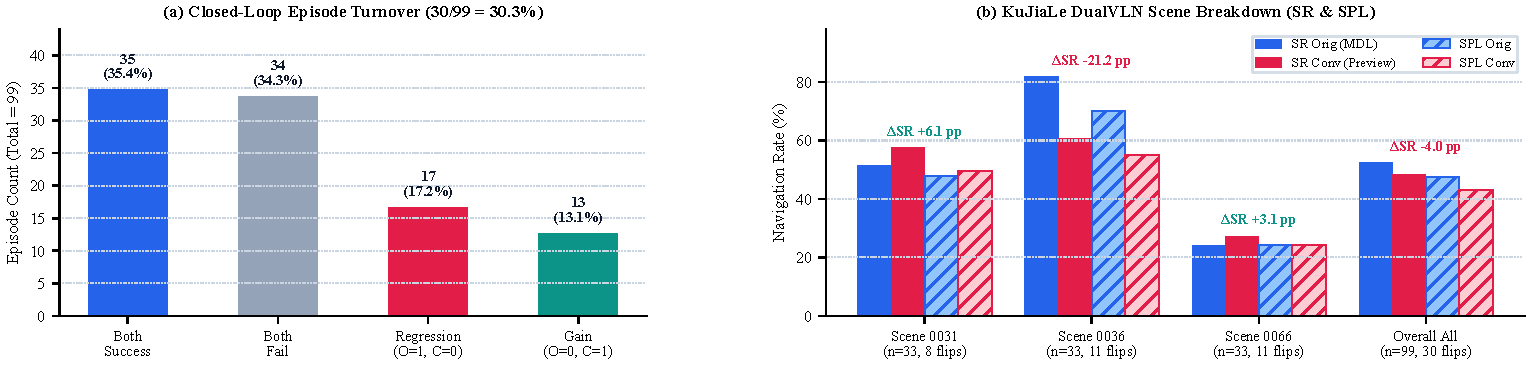
\includegraphics[width=\textwidth]{fig6_navigation_vln.pdf}
\caption{\textbf{Closed-loop \textsc{InternNav/DualVLN} navigation outcome redistribution over 99 paired episodes (\textbf{RQ4}).}
\emph{(a)} Aggregate outcome transitions: 17 success-to-failure losses and 13 failure-to-success gains yield 30 changed episode outcomes ($30.3\%$ turnover) despite only a $-4.0$ percentage-point net \textsc{SR} shift ($52.5\% \to 48.5\%$).
\emph{(b)} Scene-level \textsc{SR} and \textsc{SPL} breakdown across scenes \texttt{0031}, \texttt{0036}, and \texttt{0066}.}
\label{fig:navigation}
\end{figure*}

\paragraph{Bidirectional outcome redistribution across trajectories}
Table~\ref{tab:navigation} and Figure~\ref{fig:navigation} reveal the same aggregate cancellation pattern observed in single-frame grounding, amplified over multi-step closed-loop rollouts. Aggregate \textsc{SR} moves modestly from \NavSrOriginal\% ($52/99$) to \NavSrConverted\% ($48/99$, net $-4.0$ pp), while mean \textsc{NE} ($3.680 \to 3.631$) and \textsc{TL} ($6.975 \to 7.060$) barely change. At the episode level, however, \NavFlips/\NavN\ episodes (\NavFlipPercent\%) change final binary status: 17 previously successful episodes fail while 13 previously unsuccessful episodes succeed. Scene \texttt{0036} suffers the sharpest drop ($81.8\% \to 60.6\%$ \textsc{SR}, $-15.0$ pp \textsc{SPL}), whereas scenes \texttt{0031} and \texttt{0066} show net increases ($+6.1$ pp and $+3.1$ pp \textsc{SR}). Fresh simulator load profiling across 18 launches (\ref{app:navigation}) confirms comparable initialization timing and GPU memory utilization under both shader pipelines.

\paragraph{Qualitative trajectory divergence}
Figure~\ref{fig:trajectories} presents ending observations and top-down path overlays from dedicated qualitative video recordings of three paired episodes (expanded to 12 paired recordings in \ref{app:navigation}). Early visual discrepancies near reflective doorways and hallways compound across action steps, shifting turn selection and triggering premature or delayed \texttt{STOP} decisions. Together with Table~\ref{tab:navigation}, these trajectories illustrate how shader-level changes alter sequential control; isolating shader effects from multi-run simulator variance across repeated closed-loop rollouts remains a practical direction noted in Section~\ref{sec:conclusion}.

\begin{figure}[!t]
\centering
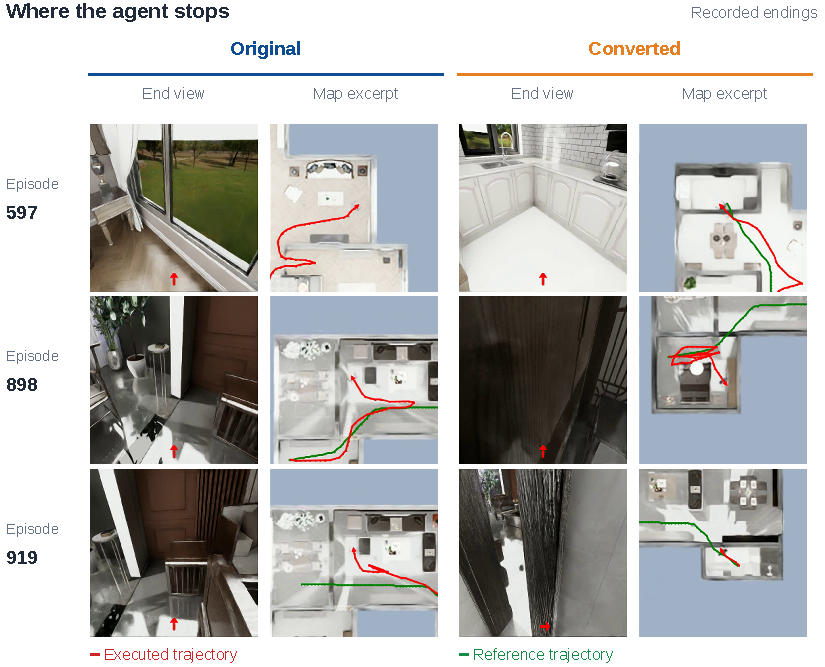
\includegraphics[width=\linewidth]{trajectories.pdf}
\caption{Qualitative ending views and top-down trajectory excerpts from separate video reruns sharing episode IDs with the 99-pair evaluation. Red and green paths trace executed and reference trajectories.}
\label{fig:trajectories}
\end{figure}

\section{Discussion, Limitations, and Practical Recommendations}
\label{sec:conclusion}

Across 30 indoor scenes, four VLM families, and 99 closed-loop navigation episodes, our empirical evidence points to a straightforward principle for 3D simulation pipelines: \textbf{geometric fidelity does not ensure decision fidelity}, even under invariant meshes, cameras, prompts, and deterministic greedy decoding ($0.00\%$ repeat variance). Lowering \textsc{MDL} shader networks to \usdps{} reverses $4.17\%\text{--}23.13\%$ of single-frame localizations across \textsc{Qwen3-VL-2B/8B/32B}, \textsc{InternVL3.5-8B-HF}, \textsc{Molmo2-8B}, and \textsc{LLaVA-NeXT-Mistral-7B}, outstripping same-material ray-tracing variance across every model while hiding behind modest dataset-wide hit deltas ($+0.42\%$ on 32B, \textsc{Molmo2-8B}, and \textsc{LLaVA-NeXT-Mistral-7B}). Across 2,880 pixel-exact counterfactuals on two 8B families, matching $\mathrm{CIE}~L^*a^*b^*$ color and luminance leaves an identical $+3.54\%$ non-photometric \textsc{BSDF} residual, arising as specular glare suppression aids metallic targets while loss of surface texture and refraction degrades sensitive queries. Because $85.7\%$ of regressions among $\ge$7B models occur on single architectures, a family-calibrated zero-\textsc{VLM} gate predicts regressions reliably ($0.743$ vs.\ $0.432$ global \textsc{RGB MAE} test \textsc{AUROC}; $0.582$ when pooled across heterogeneous checkpoints).

\paragraph{Practical recommendations for simulation pipelines}
First, converted \textsc{USD} scenes should not be signed off using dataset-level accuracy or global \textsc{RGB MAE} alone; pipelines benefit from tracking paired instance-level pass/fail IDs, locking greedy coordinate readout, and benchmarking \emph{Loss}/\emph{Gain} turnover against ray-tracing repeat floors. Second, training our lightweight zero-\textsc{VLM} risk gate per target deployment family allows export workflows to route only the highest-risk $20\%$ of views (small, peripheral, structurally flattened, or glass targets) for selective \textsc{MDL} preservation rather than sacrificing throughput on every asset.

\paragraph{Limitations and scope}
Four boundaries define the scope of this study. First, all 14,016 grounding predictions come from open-weight models whose precision and decoding states could be held uniform across local runs; proprietary API-served models lack equivalent reproducibility guarantees. Second, object queries and simulator masks were validated against ground-truth simulator geometry rather than human psychophysical annotations. Third, pixel-exact compositing isolates primary shader transitions cleanly without fresh ray-tracing jitter, while indirect multi-bounce lighting interactions remain coupled in the full converted renders ($I^F$). Finally, whereas our static grounding suite tightly bounds greedy and rendering noise, the 99-episode closed-loop navigation study executes single rollouts per condition; quantifying multi-seed simulator run variance over sequential trajectories remains a natural next step.

\section*{CRediT Authorship Contribution Statement}
\textbf{Zihou Zhu:} Conceptualization, Methodology, Software, Validation, Formal analysis, Investigation, Data curation, Visualization, Writing -- original draft, Writing -- review \& editing.

\section*{Declaration of Competing Interest}
The author declares that they have no known competing financial interests or personal relationships that could have appeared to influence the work reported in this paper.

\section*{Data Availability}
The paired scene renders, simulator segmentation masks, model prediction logs, and analysis scripts supporting the findings of this study will be made publicly available upon publication.

\section*{Declaration of generative AI and AI-assisted technologies in the writing process}
During the preparation of this work the author used large language model coding and writing assistants (Claude and Gemini) in order to assist with analysis and visualization scripting and to improve the language and readability of the manuscript. All experimental scene renders, simulator segmentation masks, closed-loop navigation rollouts, and model predictions originate directly from recorded simulator executions and deterministic model evaluations. After using these tools, the author reviewed, verified, and edited the content and code as needed and takes full responsibility for the content of the published article.

\bibliographystyle{elsarticle-harv}
\bibliography{references}
\clearpage\appendix
% Extended evidence, organized cleanly in continuous two-column flow.
\makeatletter
\setlength{\@fptop}{0pt}
\makeatother
\setcounter{topnumber}{3}
\setcounter{bottomnumber}{2}
\setcounter{totalnumber}{4}
\setcounter{dbltopnumber}{2}
\renewcommand{\topfraction}{0.88}
\renewcommand{\bottomfraction}{0.80}
\renewcommand{\textfraction}{0.10}
\renewcommand{\floatpagefraction}{0.84}
\renewcommand{\dbltopfraction}{0.88}
\renewcommand{\dblfloatpagefraction}{0.84}
\setlength{\textfloatsep}{7pt plus 2pt minus 2pt}
\setlength{\dbltextfloatsep}{8pt plus 2pt minus 2pt}
\setlength{\floatsep}{6pt plus 2pt minus 2pt}
\setlength{\dblfloatsep}{6pt plus 2pt minus 2pt}

\section{Conversion and the Appearance of the Input}
\label{app:details}
\label{app:appearance}

\begin{figure*}[!t]
\centering
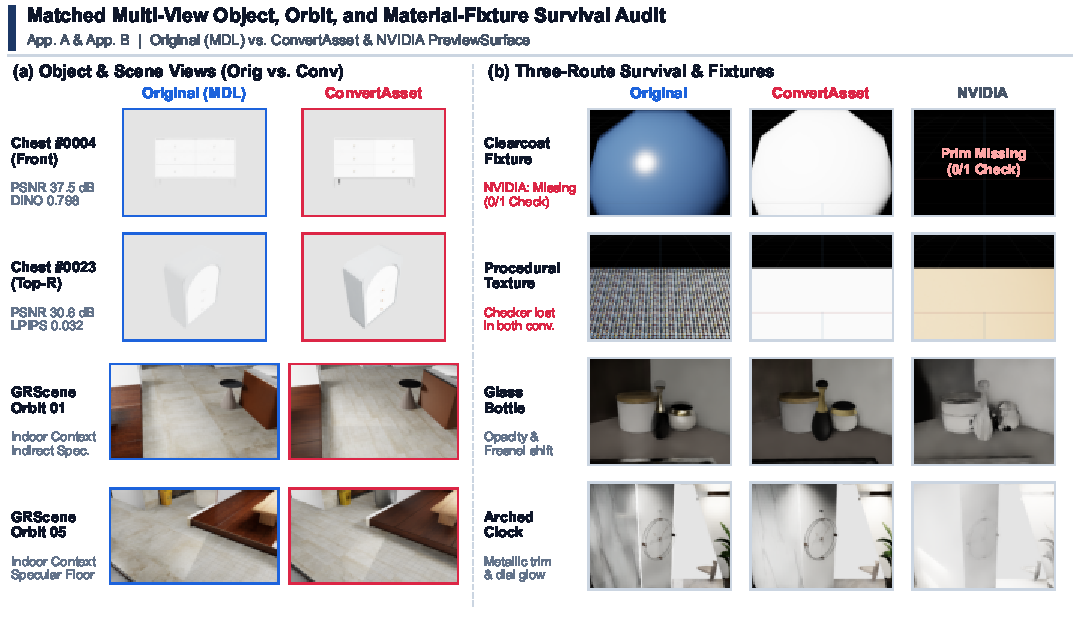
\includegraphics[width=\textwidth]{app_fig1_appearance_and_materials.pdf}
\caption{\textbf{Controlled multi-view appearance metrics and three-route material fixture survival.}
\emph{(a)} Representative paired renders between native \textsc{NVIDIA MDL} (\original{}) and lowered \usdps{} (\converted{}) across four-asset multi-view chest-of-drawers renders (reported quantitatively in Table~\ref{tab:app-proxy}) and \textsc{GRScenes} scene orbits preserving room context and indirect reflections.
\emph{(b)} Side-by-side survival comparison across \original{}, \textsc{ConvertAsset}, and the \textsc{NVIDIA} preview conversion baseline covering diagnostic fixtures (clearcoat and procedural checker) and paired \textsc{GRScenes} targets (Section~\ref{app:materials} and Table~\ref{tab:app-materials}).}
\label{fig:app-appearance-materials}
\end{figure*}

Material translation alters surface shading networks while preserving scene meshes, object transforms, camera parameters, and lighting placement. In particular, \textsc{ConvertAsset} recursively traverses \textsc{USD} references, payloads, sublayers, and variant sets, writing sibling converted layers whose bindings target \usdps{} counterparts while leaving the source \textsc{MDL} scenes unmodified. Base color, roughness, metallic response, normal maps, and texture connections are mapped explicitly, whereas higher-order clearcoat, transmission, and procedural shaders require coarse approximations (detailed further in~\ref{app:materials}).

\subsection{Matched multi-view object appearance}
To isolate multi-view perceptual fidelity prior to indoor scene evaluation, four chest-of-drawers assets from a preliminary toolkit benchmark \citep{Zhu2026Evaluating} are each rendered from six canonical camera angles (front, back, left, right, and two elevated front views), yielding 24 paired renders (Table~\ref{tab:app-proxy}). Pixel error uses $\mathrm{PSNR} = 10\log_{10}(1/\mathrm{MSE})$ on $[0,1]$-scaled RGB frames; structural similarity uses $\mathrm{SSIM}$ \citep{Wang2004Image}; perceptual distance uses \textsc{VGG}-backbone $\mathrm{LPIPS}$ \citep{Zhang2018Unreasonable}; and semantic feature cosine similarity $f(I^O)^\top f(I^C)/(\|f(I^O)\|_2\|f(I^C)\|_2)$ uses \textsc{CLIP} ViT-B/32 \citep{Radford2021Learning} and \textsc{DINOv2} \citep{Oquab2023DINOv2}.

\begin{table}[!htbp]
\centering\small
\resizebox{\linewidth}{!}{% Generated by appendix/build_tables.py; source hashes in table_sources.json.
\begin{tabular}{lrrrrrr}
\toprule
Asset & Pairs & PSNR & SSIM & LPIPS & CLIP & DINOv2 \\
\midrule
Chest 0004 & 6 & 37.51 & 0.991 & 0.019 & 0.921 & 0.798 \\
Chest 0011 & 6 & 36.30 & 0.993 & 0.017 & 0.956 & 0.922 \\
Chest 0023 & 6 & 30.59 & 0.986 & 0.032 & 0.938 & 0.905 \\
Chest 0029 & 6 & 37.68 & 0.991 & 0.014 & 0.885 & 0.864 \\
All & 24 & 35.52 & 0.990 & 0.020 & 0.925 & 0.872 \\
\bottomrule
\end{tabular}
}
\caption{Matched object renders averaged over six camera directions per asset. Higher PSNR (dB), SSIM, CLIP, and DINOv2 indicate stronger visual similarity; lower LPIPS indicates closer perceptual match.}
\label{tab:app-proxy}
\end{table}

Aggregate fidelity across all 24 views is high ($\mathrm{PSNR}=35.52\,\mathrm{dB}$, $\mathrm{SSIM}=0.990$, $\mathrm{LPIPS}=0.020$), yet per-asset profiles diverge meaningfully: Chest~0023 records the lowest PSNR ($30.59\,\mathrm{dB}$) and highest LPIPS ($0.032$), whereas Chest~0004 records the lowest DINOv2 similarity ($0.798$) despite high PSNR ($37.51\,\mathrm{dB}$). Figure~\ref{fig:app-appearance-materials}(a) places the chest views alongside indoor \textsc{GRScenes} camera orbits, illustrating why holistic object metrics still allow localized changes in specular reflections, wood sheen, and nearby surface lighting.

\section{Material-Effect Survival Under Conversion}
\label{app:materials}

Table~\ref{tab:app-materials} and Figure~\ref{fig:app-appearance-materials}(b) compare native \textsc{NVIDIA MDL}, \textsc{ConvertAsset}, and the \textsc{NVIDIA} \usdps{} conversion baseline across four \textsc{GRScenes} effect groups (opacity/transparency, emission, normal/bump mapping, and displacement/height) plus two synthetic stress fixtures (clearcoat and procedural checker textures). Because natural scenes exhibit overlapping shader effects, static effect counts overlap across groups.

\begin{table}[!htbp]
\centering\small
\resizebox{\linewidth}{!}{% Generated by appendix/build_tables.py; source hashes in table_sources.json.
\begin{tabular}{lrrrr}
\toprule
Effect & $N$ & Original & ConvertAsset & NVIDIA \\
\midrule
Clearcoat fixture & 1 & 1/1 & 1/1 & 0/1 \\
Opacity / transparency & 7 & 7/7 & 7/7 & 7/7 \\
Emission & 26 & 26/26 & 26/26 & 26/26 \\
Procedural fixture & 1 & 1/1 & 1/1 & 1/1 \\
Normal / bump & 30 & 30/30 & 30/30 & 30/30 \\
Displacement / height & 26 & 26/26 & 26/26 & 26/26 \\
\bottomrule
\end{tabular}
}
\caption{Static material-effect survival inventory across native \textsc{MDL}, \textsc{ConvertAsset}, and the \textsc{NVIDIA} baseline (checks verify target prim presence and zero remaining active \textsc{MDL}).}
\label{tab:app-materials}
\end{table}

All four \textsc{GRScenes} effect groups produce statically valid USD outputs under both conversion routes, yet paired renders in Figure~\ref{fig:app-appearance-materials}(b) reveal distinct visual failure modes masked by static structural checks:
\begin{itemize}
    \item \textbf{Clearcoat structural drop vs.\ approximation.} On the controlled clearcoat fixture, the \textsc{NVIDIA} converter fails to preserve the target prim ($0/1$ static check), whereas \textsc{ConvertAsset} preserves target geometry ($1/1$) while flattening the secondary coat lobe into a higher-albedo surface response.
    \item \textbf{Procedural pattern loss under valid USD bindings.} On the procedural checker fixture, both converted outputs pass all static graph and binding checks ($1/1$), yet the fine high-frequency checkerboard disappears completely into a uniform base surface.
    \item \textbf{Scene-embedded glass and metallic fixtures.} Across the natural bottle and arched clock captures, \textsc{ConvertAsset} preserves global silhouette and room illumination more faithfully than the washed \textsc{NVIDIA} route, while still stripping secondary specular highlights and Fresnel contrast that alter \textsc{VLM} localization.
\end{itemize}

\section{Scene Catalog and Controlled Two-View Ablation}
\label{app:construction}

\begin{figure*}[!t]
\centering
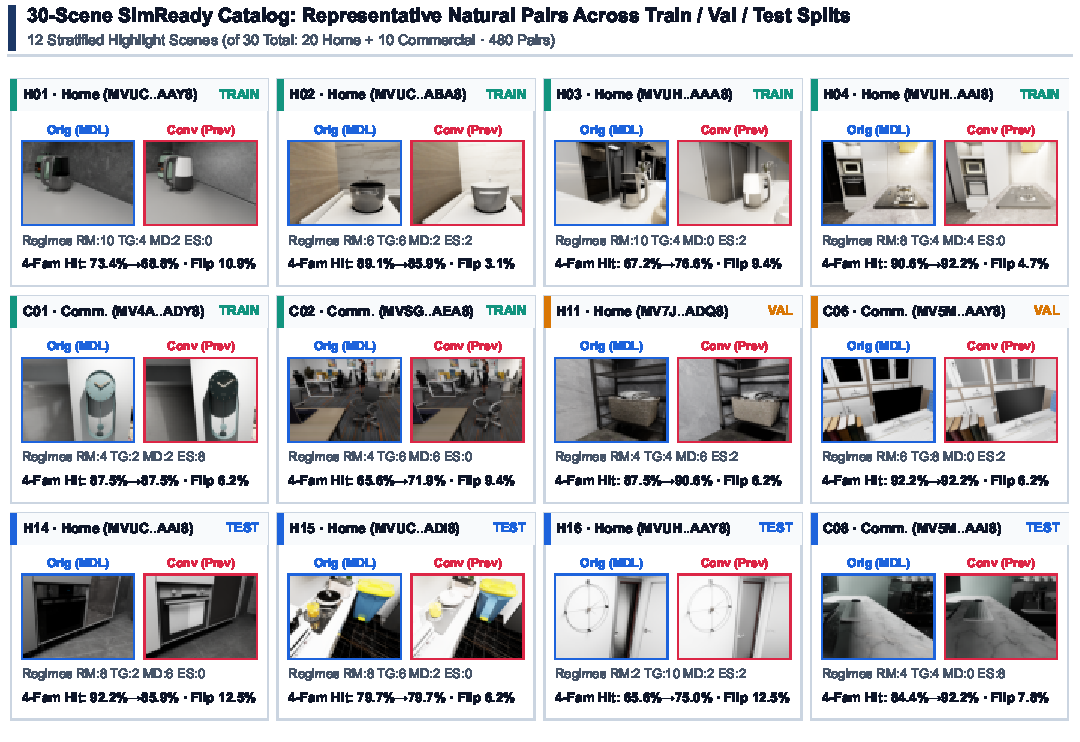
\includegraphics[width=0.94\textwidth]{app_fig2_scene30_atlas.pdf}
\caption{\textbf{Stratified catalog of the 30-scene \textsc{SimReady GRScenes} grounding benchmark.}
Twelve representative scenes spanning \texttt{Train} (15 scenes total), \texttt{Val} (5 scenes), and \texttt{Test} (10 scenes) across residential (\texttt{home\_scenes}, \texttt{H01--H20}) and commercial (\texttt{commercial\_scenes}, \texttt{C01--C10}) environments. Each card pairs canonical \original{} (\textsc{MDL}) and \converted{} (\usdps{}) captures, optical-regime composition (\texttt{RM/TG/MD/ES}), and four-family mean accuracy shift and decision flip rate; the full 30-scene breakdown appears in Table~\ref{tab:app-scenes30}.}
\label{fig:app-scene30}
\end{figure*}

\begin{table*}[!t]
\centering
\caption{Complete per-scene breakdown across all 30 independent \textsc{GRScenes} assets ($16$ camera pairs per scene; $480$ total pairs). Entries under each model report $H_O/H_C~(\mathrm{Flip\%})$ under deterministic greedy ($T{=}0$) evaluation; $\mathrm{SSIM}$ and $\Delta L^*$ report mean target-mask structural similarity and lightness shift.}
\label{tab:app-scenes30}
\resizebox{\textwidth}{!}{% Generated automatically by build_cviu_appendix_assets.py from pair_optical_features.json and v3 predictions
\begin{tabular}{@{}llllcrrrrrrr@{}}
\toprule
Code & Scene ID & Dom. & Split & RM/TG/MD/ES & SSIM & $\Delta L^*$ & Qwen3-8B & Qwen3-32B & InternVL3.5 & Molmo2-8B & LLaVA-7B \\
\midrule
H01 & \texttt{MVUC..AAY8} & Home & Train & 10/4/2/0 & 0.66 & 8.0 & 62/62 (12.5) & 81/81 (0.0) & 75/69 (6.2) & 100/100 (0.0) & 56/44 (25.0) \\
H02 & \texttt{MVUC..ABA8} & Home & Train & 6/6/2/2 & 0.66 & 10.6 & 88/88 (0.0) & 88/100 (12.5) & 88/81 (6.2) & 100/100 (0.0) & 81/75 (6.2) \\
H03 & \texttt{MVUH..AAA8} & Home & Train & 10/4/0/2 & 0.57 & 13.3 & 62/75 (12.5) & 88/81 (6.2) & 62/75 (12.5) & 94/94 (0.0) & 50/62 (12.5) \\
H04 & \texttt{MVUH..AAI8} & Home & Train & 8/4/4/0 & 0.73 & 5.4 & 94/94 (0.0) & 100/100 (0.0) & 81/88 (18.8) & 100/100 (0.0) & 88/88 (0.0) \\
H05 & \texttt{MVUH..AAI8} & Home & Train & 4/8/4/0 & 0.75 & 7.4 & 94/94 (12.5) & 94/94 (12.5) & 81/88 (6.2) & 88/100 (12.5) & 75/44 (31.2) \\
H06 & \texttt{MWAX..AAA8} & Home & Train & 10/4/2/0 & 0.56 & 13.4 & 81/88 (18.8) & 94/94 (0.0) & 81/88 (6.2) & 100/88 (12.5) & 56/56 (25.0) \\
H07 & \texttt{MWAX..ADA8} & Home & Train & 6/0/4/6 & 0.69 & 13.6 & 100/100 (0.0) & 100/100 (0.0) & 88/94 (6.2) & 88/88 (0.0) & 94/94 (0.0) \\
H08 & \texttt{MWAX..AEA8} & Home & Train & 8/2/6/0 & 0.74 & 9.8 & 100/100 (0.0) & 94/94 (0.0) & 75/75 (25.0) & 100/100 (0.0) & 81/81 (12.5) \\
H09 & \texttt{MWBG..ABA8} & Home & Train & 4/10/2/0 & 0.54 & 11.2 & 100/88 (12.5) & 100/100 (0.0) & 69/69 (12.5) & 94/100 (6.2) & 50/50 (12.5) \\
H10 & \texttt{MWBG..ABI8} & Home & Train & 4/2/6/4 & 0.73 & 15.5 & 81/88 (6.2) & 100/100 (0.0) & 88/94 (6.2) & 100/100 (0.0) & 62/69 (18.8) \\
C01 & \texttt{MV4A..ADY8} & Comm & Train & 4/2/2/8 & 0.65 & 7.1 & 88/94 (6.2) & 88/94 (6.2) & 88/88 (0.0) & 100/100 (0.0) & 75/69 (18.8) \\
C02 & \texttt{MVSG..AEA8} & Comm & Train & 4/6/6/0 & 0.74 & 4.9 & 50/56 (18.8) & 81/75 (6.2) & 75/81 (6.2) & 75/81 (6.2) & 62/69 (6.2) \\
C03 & \texttt{MWF4..ACI8} & Comm & Train & 4/12/0/0 & 0.71 & 8.9 & 75/81 (6.2) & 88/88 (0.0) & 81/81 (12.5) & 94/94 (0.0) & 88/88 (0.0) \\
C04 & \texttt{MWF4..ADI8} & Comm & Train & 0/6/2/8 & 0.63 & 10.2 & 69/69 (12.5) & 94/100 (6.2) & 69/75 (31.2) & 94/100 (6.2) & 50/62 (25.0) \\
C05 & \texttt{MWF4..ADQ8} & Comm & Train & 4/10/2/0 & 0.69 & 6.0 & 75/81 (6.2) & 75/81 (6.2) & 69/69 (12.5) & 94/100 (6.2) & 50/56 (56.2) \\
\midrule
H11 & \texttt{MV7J..ADQ8} & Home & Val & 4/4/6/2 & 0.71 & 6.9 & 94/94 (0.0) & 100/100 (0.0) & 94/100 (6.2) & 100/100 (0.0) & 62/69 (18.8) \\
H12 & \texttt{MV7J..ADY8} & Home & Val & 8/6/2/0 & 0.56 & 11.2 & 88/94 (6.2) & 100/100 (0.0) & 94/94 (12.5) & 100/100 (0.0) & 75/81 (18.8) \\
H13 & \texttt{MV7J..AEA8} & Home & Val & 2/8/2/4 & 0.52 & 17.5 & 94/88 (18.8) & 100/100 (0.0) & 88/88 (25.0) & 88/88 (12.5) & 75/62 (37.5) \\
C06 & \texttt{MV5M..AAY8} & Comm & Val & 6/8/0/2 & 0.75 & 5.5 & 94/94 (12.5) & 100/100 (0.0) & 88/94 (6.2) & 100/100 (0.0) & 88/81 (6.2) \\
C07 & \texttt{MVSY..ACY8} & Comm & Val & 4/4/6/2 & 0.66 & 3.3 & 62/69 (18.8) & 69/81 (12.5) & 56/62 (6.2) & 75/75 (25.0) & 50/56 (31.2) \\
\midrule
H14 & \texttt{MVUC..AAI8} & Home & Test & 8/2/6/0 & 0.61 & 11.8 & 94/88 (18.8) & 94/100 (6.2) & 94/81 (12.5) & 100/88 (12.5) & 81/88 (6.2) \\
H15 & \texttt{MVUC..ADI8} & Home & Test & 8/6/2/0 & 0.65 & 14.0 & 75/81 (6.2) & 100/94 (6.2) & 75/69 (6.2) & 100/100 (0.0) & 69/69 (12.5) \\
H16 & \texttt{MVUH..AAY8} & Home & Test & 2/10/2/2 & 0.64 & 5.3 & 69/75 (18.8) & 94/88 (6.2) & 62/69 (6.2) & 88/88 (0.0) & 44/69 (25.0) \\
H17 & \texttt{MVUH..ACQ8} & Home & Test & 4/6/4/2 & 0.47 & 5.4 & 62/75 (12.5) & 88/81 (6.2) & 69/62 (31.2) & 100/94 (6.2) & 31/38 (18.8) \\
H18 & \texttt{MVUH..ADA8} & Home & Test & 4/10/2/0 & 0.58 & 10.8 & 100/100 (0.0) & 94/94 (0.0) & 94/88 (6.2) & 100/100 (0.0) & 81/75 (18.8) \\
H19 & \texttt{MWAX..ADQ8} & Home & Test & 2/10/4/0 & 0.65 & 6.3 & 81/81 (12.5) & 100/100 (0.0) & 94/94 (0.0) & 100/100 (0.0) & 94/81 (12.5) \\
H20 & \texttt{MWBG..ACA8} & Home & Test & 6/4/4/2 & 0.60 & 17.1 & 81/81 (0.0) & 100/94 (6.2) & 75/75 (0.0) & 94/100 (6.2) & 50/56 (6.2) \\
C08 & \texttt{MV5M..AAI8} & Comm & Test & 4/4/0/8 & 0.76 & 2.7 & 75/88 (12.5) & 100/94 (6.2) & 75/81 (6.2) & 100/100 (0.0) & 88/100 (12.5) \\
C09 & \texttt{MWF4..ACY8} & Comm & Test & 2/12/2/0 & 0.59 & 6.4 & 94/88 (6.2) & 94/94 (0.0) & 81/81 (12.5) & 94/81 (12.5) & 56/50 (18.8) \\
C10 & \texttt{MWF4..AEA8} & Comm & Test & 8/2/2/4 & 0.60 & 8.0 & 56/44 (12.5) & 56/62 (18.8) & 50/50 (12.5) & 62/75 (12.5) & 62/56 (6.2) \\
\midrule
\textbf{All 30} & \textbf{480 pairs} & 20H/10C & 15/5/10 & \textbf{158/176/88/58} & \textbf{0.65} & \textbf{9.2} & \textbf{81.2/83.1 (9.4)} & \textbf{91.7/92.1 (4.2)} & \textbf{78.5/80.0 (10.6)} & \textbf{94.0/94.4 (4.6)} & \textbf{67.5/67.9 (16.7)} \\
\bottomrule
\end{tabular}
}
\end{table*}

\subsection{30-scene SimReady composition and mask integrity}
The 30-scene benchmark consists of \textbf{30 independent SimReady scenes} from \textsc{GRScenes} ($20$ residential \texttt{H01--H20} and $10$ commercial \texttt{C01--C10}), split at the scene level prior to feature fitting into \textbf{15 training (240 pairs), 5 validation (80 pairs), and 10 held-out test scenes (160 pairs)}. Within each scene, eight visible object instances are captured from two natural viewpoints at $1024{\times}768$, giving $240$ targets and $480$ paired captures ($960$ images), alongside three stratified control scenes ($48$ pairs) rendered across three independent path-tracing repeats under locked geometry and \textsc{MDL} materials. Figure~\ref{fig:app-scene30} depicts twelve representative scene cards, and Table~\ref{tab:app-scenes30} summarizes optical regimes and per-model turnover across all 30 scenes. Commercial scenes frequently match or exceed residential turnover across specialist and general models alike (e.g., \texttt{C10} flips $12.5\%$ even on \textsc{Molmo2-8B} and $18.8\%$ on \textsc{Qwen3-VL-32B}), indicating that shader-induced sensitivity extends well beyond domestic interiors.

\subsection{Controlled two-view gutter ablation}
\label{app:early_canvas}
In a supplementary controlled two-view ablation isolating four individual objects (bottle, clock, cup, and backpack), paired object captures were arranged cyclically across a 16-pixel neutral gray gutter on $(2W{+}16)\times H$ canvases in both left/right placements ($4{\times}2{\times}2 = 16$ queries per condition). Placing the frame midpoint inside the empty gutter rules out center-bias guessing, while target-window, context-window, and full-canvas crossovers built from integer bounding boxes motivate both the pixel-exact simulator masks $M_i^v$ and natural camera framing used in the main 30-scene benchmark.

\section{Spatial Readout Interface and Qualification Gate}
\label{app:readout}

\begin{figure*}[!t]
\centering
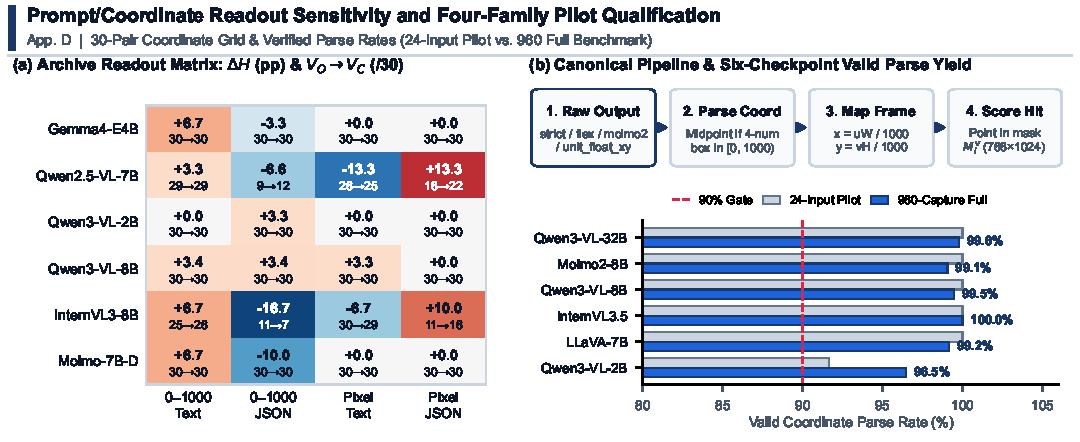
\includegraphics[width=0.95\textwidth]{app_fig3_readout_and_pilot.pdf}
\caption{\textbf{Spatial readout frame sensitivity and four-family pilot qualification.}
\emph{(a)} Archive heatmap of paired score deltas $\Delta H = H_C - H_O$ (percentage points) and valid numeric parse counts $(V_O \to V_C / 30)$ across normalized $0\text{--}1000$ vs.\ pixel frames and text vs.\ JSON prompts (full values in Table~\ref{tab:protocol-full}).
\emph{(b)} Canonical four-step \texttt{Parse $\to$ Align $\to$ Score} pipeline (top) and verified valid coordinate parse rates on both the isolated 24-input pilot qualification gate ($\ge 90\%$) and full 960-capture 30-scene benchmark ($96.5\%\text{--}100.0\%$ across all six evaluated checkpoints).}
\label{fig:app-readout-pilot}
\end{figure*}

Inconsistent prompt schemas or coordinate conventions can easily masquerade as optical sensitivity. Figure~\ref{fig:app-readout-pilot}(a) and Table~\ref{tab:protocol-full} evaluate six model configurations on fixed 30-pair target-centered captures across a $2{\times}2$ interface matrix crossing frame requests ($0\text{--}1000$ normalized vs.\ image pixels) and response schemas (two-line text \texttt{Point:\ x, y} vs.\ JSON \texttt{point\_xy}). A parsed point counts toward valid parse coverage $V$ even when falling outside image bounds, whereas a hit $H$ requires landing inside the target region.

\begin{table}[!htbp]
\centering\small
\setlength{\tabcolsep}{3pt}
\resizebox{\linewidth}{!}{% Generated by scripts/build_assets.py from corrected results.json
\begin{tabular}{lllrrrr}
\toprule
Model & Frame & Format & $V_O$ & $V_C$ & $H_O$ (\%) & $H_C$ (\%) \\
\midrule
Gemma4-E4B & 0--1000 & text & 30/30 & 30/30 & 90.0 & 96.7 \\
Gemma4-E4B & 0--1000 & JSON & 30/30 & 30/30 & 90.0 & 86.7 \\
Gemma4-E4B & pixel & text & 30/30 & 30/30 & 36.7 & 36.7 \\
Gemma4-E4B & pixel & JSON & 30/30 & 30/30 & 0.0 & 0.0 \\
Qwen2.5-VL-7B & 0--1000 & text & 29/30 & 29/30 & 10.0 & 13.3 \\
Qwen2.5-VL-7B & 0--1000 & JSON & 9/30 & 12/30 & 13.3 & 6.7 \\
Qwen2.5-VL-7B & pixel & text & 26/30 & 25/30 & 80.0 & 66.7 \\
Qwen2.5-VL-7B & pixel & JSON & 18/30 & 22/30 & 60.0 & 73.3 \\
Qwen3-VL-2B & 0--1000 & text & 30/30 & 30/30 & 86.7 & 86.7 \\
Qwen3-VL-2B & 0--1000 & JSON & 30/30 & 30/30 & 90.0 & 93.3 \\
Qwen3-VL-2B & pixel & text & 30/30 & 30/30 & 60.0 & 60.0 \\
Qwen3-VL-2B & pixel & JSON & 30/30 & 30/30 & 0.0 & 0.0 \\
Qwen3-VL-8B & 0--1000 & text & 30/30 & 30/30 & 93.3 & 96.7 \\
Qwen3-VL-8B & 0--1000 & JSON & 30/30 & 30/30 & 93.3 & 96.7 \\
Qwen3-VL-8B & pixel & text & 30/30 & 30/30 & 0.0 & 3.3 \\
Qwen3-VL-8B & pixel & JSON & 30/30 & 30/30 & 0.0 & 0.0 \\
InternVL3-8B & 0--1000 & text & 25/30 & 26/30 & 60.0 & 66.7 \\
InternVL3-8B & 0--1000 & JSON & 11/30 & 7/30 & 36.7 & 20.0 \\
InternVL3-8B & pixel & text & 30/30 & 29/30 & 16.7 & 10.0 \\
InternVL3-8B & pixel & JSON & 11/30 & 16/30 & 10.0 & 20.0 \\
Molmo-7B-D & 0--1000 & text & 30/30 & 30/30 & 90.0 & 96.7 \\
Molmo-7B-D & 0--1000 & JSON & 30/30 & 30/30 & 13.3 & 3.3 \\
Molmo-7B-D & pixel & text & 30/30 & 30/30 & 0.0 & 0.0 \\
Molmo-7B-D & pixel & JSON & 30/30 & 30/30 & 0.0 & 0.0 \\
\bottomrule
\end{tabular}
}
\caption{Coordinate-frame and schema ablation on the 30-pair multi-view set. $V$ counts parsed numeric points over 30 queries; $H$ reports end-to-end hit percentage under the requested frame.}
\label{tab:protocol-full}
\end{table}

Frame mismatches distort apparent performance substantially: requesting pixel output from \textsc{Qwen3-VL-8B} or \textsc{Molmo-7B-D} while the model emits $0\text{--}1000$ coordinates reduces hit rates from $90.0\%\text{--}96.7\%$ to $0.0\%\text{--}3.3\%$, whereas \textsc{Qwen2.5-VL-7B} prefers pixels ($80.0\%$ pixel text vs.\ $10.0\%$ normalized text). For frame size $K$, mapping $(u,v) \mapsto (uW/K, vH/K)$ under a fixed query denominator prevents format errors from masquerading as visual improvements or regressions.

\subsection{Scorer verification on coordinate-only baselines}
Deterministic sanity checks on the 30-pair multi-view captures verify frame alignment: a fixed image-center baseline scores $30/30$ in pixels but $0/30$ under $[0, 1000)$ normalization; an oracle box center reaches $30/30$ only when emitted and evaluated in matching frames; and a seeded random pixel baseline hits $5/30$ (\original) and $2/30$ (\converted) under pixels versus $8/30$ and $3/30$ when normalized. These checks motivate both the canonical $[0, 1000)$ interface and off-center framing across the 30-scene suite.

\subsection{Four-family pilot qualification and calibrated parsers}
Prior to 30-scene evaluation, every checkpoint passed an isolated 24-input pilot qualification gate ($\ge 90\%$ valid parse yield; Figure~\ref{fig:app-readout-pilot}(b) and Table~\ref{tab:app-pilot-v3}) that fixed one deterministic parser mode per family:
\begin{itemize}
    \item \texttt{strict}: exact \texttt{Point:\ x, y} line in $[0, 1000)$ (\textsc{Qwen3-8B/32B} and \textsc{InternVL3.5}; $100\%$ pilot, $\ge 99.5\%$ full).
    \item \texttt{flex\_1000}: handles \textsc{Qwen3-VL-2B}'s bare \texttt{(x, y)} tuples, JSON \texttt{point\_2d}, and 4-number box midpoints without corner truncation ($91.7\%$ pilot, $96.5\%$ full).
    \item \texttt{molmo2\_1000}: parses \textsc{Molmo2-8B}'s native \texttt{<points coords="1 1 x y">} and \texttt{<Point:\ x y>} tags directly in $[0, 1000]$ ($100.0\%$ pilot, $99.1\%$ full).
    \item \texttt{unit\_float\_xy}: converts \textsc{LLaVA-NeXT-Mistral-7B}'s native unit-normalized $[0, 1]$ bounding-box midpoints and point tuples to $[0, 1000)$ ($100.0\%$ pilot, $99.2\%$ full).
\end{itemize}

\begin{table}[!htbp]
\centering\small
\resizebox{\linewidth}{!}{%
\begin{tabular}{@{}llrrr@{}}
\toprule
Checkpoint & Parser Mode & Pilot Valid & Pilot Hit & Full Valid ($960$) \\
\midrule
\textsc{Qwen3-VL-32B} & \texttt{strict} & 24/24 (100\%) & 20/24 (83.3\%) & 99.8\% \\
\textsc{Molmo2-8B} & \texttt{molmo2\_1000} & 24/24 (100\%) & 24/24 (100\%) & 99.1\% \\
\textsc{Qwen3-VL-8B} & \texttt{strict} & 24/24 (100\%) & 22/24 (91.7\%) & 99.5\% \\
\textsc{InternVL3.5-8B-HF} & \texttt{strict} & 24/24 (100\%) & 20/24 (83.3\%) & 100.0\% \\
\textsc{LLaVA-NeXT-Mistral-7B} & \texttt{unit\_float\_xy} & 24/24 (100\%) & 22/24 (91.7\%) & 99.2\% \\
\textsc{Qwen3-VL-2B} & \texttt{flex\_1000} & 22/24 (91.7\%) & 19/24 (79.2\%) & 96.5\% \\
\bottomrule
\end{tabular}}
\caption{Isolated 24-input pilot qualification results (all passing the $\ge 90\%$ gate under deterministic greedy decoding) and full-benchmark valid parse rates across all 960 captures.}
\label{tab:app-pilot-v3}
\end{table}

\section{Cross-Family Case Divergence and Supplementary Ablations}
\label{app:archive}

\begin{figure*}[!t]
\centering
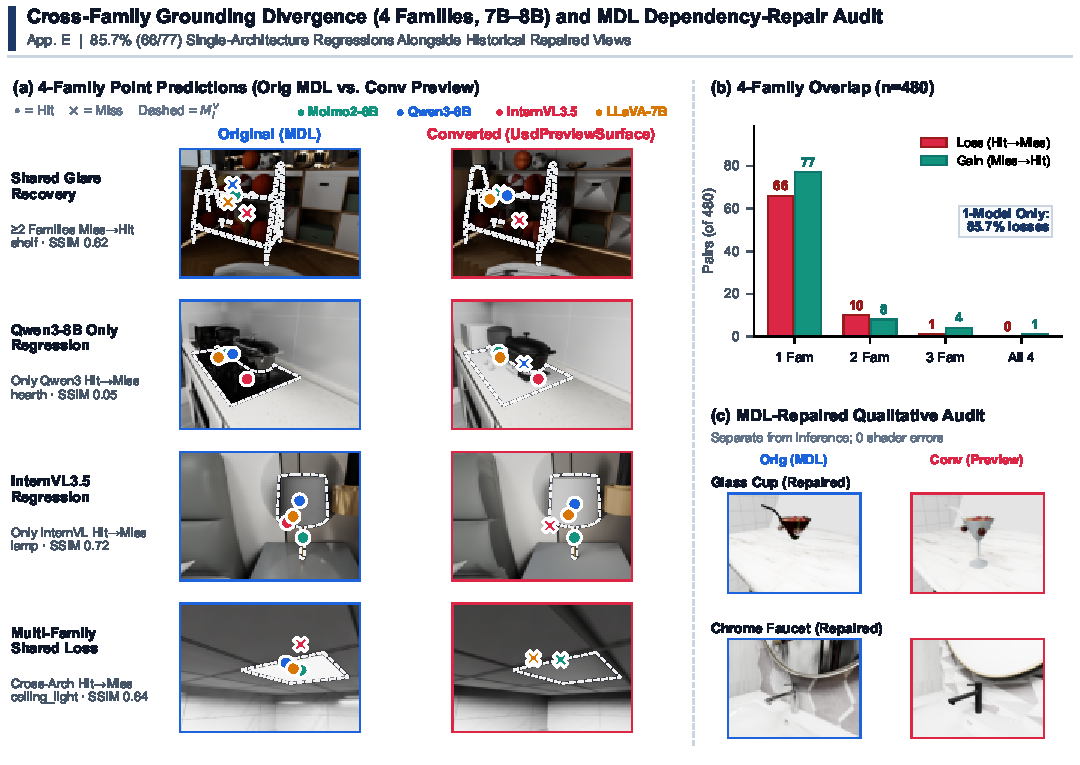
\includegraphics[width=0.92\textwidth]{app_fig4_multifamily_gallery.pdf}
\caption{\textbf{Cross-family localization divergence across 7B--8B architectures and repaired \textsc{MDL} audit.}
\emph{(a)} Representative target-centered captures across the four $\ge$7B families (\textsc{Molmo2-8B}, \textsc{Qwen3-VL-8B}, \textsc{InternVL3.5-8B-HF}, and \textsc{LLaVA-NeXT-Mistral-7B}) comparing \original{} (\textsc{MDL}) against \converted{} (\usdps{}) with simulator mask outlines $M_i^v$: shared glare recovery, architecture-unique regressions, and multi-family failures.
\emph{(b)} Distribution of how many architectures share each regression or gain across all 480 pairs ($66/77 = 85.7\%$ of regressions occur in one model only).
\emph{(c)} Representative pairs rendered after \textsc{MDL} asset dependency repair.}
\label{fig:app-multifamily}
\end{figure*}

\subsection{Architecture-specific localization failures in the 30-scene suite}
Across the four $\ge$7B families evaluated on all 480 captures, $77/480$ pairs experience at least one conversion regression (\emph{Loss}), yet \textbf{$66/77$ ($85.7\%$) of those regressions occur in only a single architecture}, $10/77$ ($13.0\%$) affect two architectures, $1/77$ ($1.3\%$) affects three, and $0/480$ cause simultaneous regression across all four families (Figure~\ref{fig:app-multifamily}(b)). Conversely, $90/480$ pairs record at least one conditional gain, with $77$ unique to a single architecture and $1$ shared across all four. Visual overlays in Figure~\ref{fig:app-multifamily}(a) illustrate why visual backbones react selectively: glare suppression helps multiple models on reflective shelves, whereas subtle contrast loss along a black glass cooktop displaces \textsc{Qwen3-VL-8B} without affecting \textsc{InternVL3.5}, and shade flattening around a table lamp affects \textsc{InternVL3.5} alone.

\subsection{Supplementary multi-view ablations}
Prior to scaling to 30 full scenes, six model configurations were evaluated across 30 close views and 80 mixed captures spanning 16 targets (Table~\ref{tab:archive}), alongside a 15-pair development split (Table~\ref{tab:app-clean15}) and 4-pair/14-pair zoom checks (Table~\ref{tab:app-historical}) scored under fixed query denominators. Retaining parse failures in the query denominator reproduces the same cancellation effect seen in the main benchmark: for example, \textsc{InternVL3-8B} gains $+5.0$~pp net accuracy over 80 views while flipping binary status on $16/80$ pairs, and \textsc{Qwen3-VL-2B} flips $13/80$ pairs around a net drop of three hits.

\begin{table}[!htbp]
\centering\small
\setlength{\tabcolsep}{3pt}
\resizebox{\linewidth}{!}{% Generated by scripts/build_assets.py from corrected results.json
\begin{tabular}{lrrrrrr}
\toprule
Model & \multicolumn{2}{c}{Close views (30)} & \multicolumn{2}{c}{Mixed views (80)} & $\Delta$ (pp) & Flips \\
\midrule
Gemma4-E4B & 90.0 & 96.7 & 70.0 & 65.0 & -5.0 & 12/80 \\
Qwen2.5-VL-7B & 10.0 & 13.3 & 3.8 & 5.0 & +1.2 & 5/80 \\
Qwen3-VL-2B & 86.7 & 86.7 & 53.8 & 50.0 & -3.8 & 13/80 \\
Qwen3-VL-8B & 93.3 & 96.7 & 86.2 & 85.0 & -1.2 & 7/80 \\
InternVL3-8B & 60.0 & 66.7 & 35.0 & 40.0 & +5.0 & 16/80 \\
Molmo-7B-D & 90.0 & 96.7 & 92.5 & 93.8 & +1.2 & 5/80 \\
\bottomrule
\end{tabular}
}
\caption{Supplementary raster readout ablation: end-to-end point hits (\%) under \original{} then \converted{}, retaining every query in the denominator.}
\label{tab:archive}
\end{table}

\begin{table}[!htbp]
\centering\small
\resizebox{\linewidth}{!}{% Generated by appendix/build_tables.py; source hashes in table_sources.json.
\begin{tabular}{lrrrrrr}
\toprule
Model & $N$ & $V_O$ & $V_C$ & $H_O$ & $H_C$ & Flips \\
\midrule
Gemma4-E4B & 15 & 15 & 15 & 8 & 6 & 4 \\
InternVL3-8B & 15 & 13 & 11 & 3 & 3 & 2 \\
Qwen2.5-VL-7B & 15 & 14 & 15 & 0 & 0 & 0 \\
Qwen3-VL-2B & 15 & 15 & 15 & 3 & 3 & 2 \\
Qwen3-VL-8B & 15 & 15 & 15 & 12 & 13 & 1 \\
\bottomrule
\end{tabular}
}
\caption{15-pair development split under normalized two-line readout ($V$ parsed outputs, $H$ hits out of $N=15$).}
\label{tab:app-clean15}
\end{table}

\subsection{Sampling temperature check and repaired MDL visual checks}
On the 30-pair multi-view set ($60$ images), three stochastic draws at $T{=}0.7$ quantify a high spatial noise floor (Table~\ref{tab:sampling}): even with $60/60$ valid parses, mean pairwise point distance ranges from $7.66\,\mathrm{px}$ (\textsc{Qwen3-VL-8B}) to $27.07\,\mathrm{px}$ (\textsc{Gemma4}), driving $10.0\%\text{--}16.7\%$ binary hit instability on \textsc{Gemma4} and \textsc{Qwen3-VL-2B}. Separately, Figure~\ref{fig:app-multifamily}(c) shows two pairs rendered after \textsc{MDL} dependency cleanup to inspect shader conversion visually. Confidence intervals in the main 30-scene evaluation resample whole scene clusters ($S{=}30$, 10,000 draws) to account for shared camera targets within scenes.

\begin{table}[!htbp]
\centering\small
\setlength{\tabcolsep}{4pt}
\resizebox{\linewidth}{!}{% Generated by appendix/build_tables.py; source hashes in table_sources.json.
\begin{tabular}{lrrrr}
\toprule
Run & $N$ & $V_O/V_C$ & Requested hits O/C & Other frame O/C \\
\midrule
Gemma4 pilot & 4 & 4/4 & 0/0 & 4/3 \\
Qwen2.5 JSON pilot & 4 & 0/0 & 0/0 & 0/0 \\
Qwen2.5 text pilot & 4 & 3/4 & 0/0 & 2/2 \\
Gemma4 zoom & 14 & 14/14 & 11/13 & 1/1 \\
Qwen2.5 zoom & 14 & 14/13 & 3/3 & 9/6 \\
\bottomrule
\end{tabular}
}
\caption{Pilot (4-pair) and zoom (14-pair) development runs rescored with fixed denominators (\original{}/\converted{}).}
\label{tab:app-historical}
\end{table}

\begin{table}[!htbp]
\centering\small
\resizebox{\linewidth}{!}{% Generated by scripts/build_assets.py from corrected results.json
\begin{tabular}{lrrr}
\toprule
Model & Complete triples & Seed distance (px) & Hit variability (\%) \\
\midrule
Qwen3-VL-8B & 60/60 & 7.66 & 0.0 \\
Qwen3-VL-2B & 60/60 & 24.34 & 16.7 \\
Gemma4-E4B & 60/60 & 27.07 & 10.0 \\
\bottomrule
\end{tabular}
}
\caption{Early stochastic decoding check ($T{=}0.7$, three draws per image across 60 archive views).}
\label{tab:sampling}
\end{table}

\section{Extended Counterfactual Stratification and Zero-VLM Risk-Gate Diagnostics}
\label{app:mechanisms_risk}

\begin{table*}[!t]
\centering
\caption{Side-by-side dual-family pixel-exact counterfactual evaluation across \textsc{Qwen3-VL-8B} ($1{,}440$ evaluations) and \textsc{InternVL3.5-8B-HF} ($1{,}440$ evaluations), spanning factorial contrasts ($480$ all vs.\ $473$ bit-identical mask subset, $\mathrm{IoU}{=}1.000$), prior optical regimes, and objective pixel-distortion groupings.}
\label{tab:app-counterfactual-dual}
\resizebox{\textwidth}{!}{% Generated automatically by build_cviu_appendix_assets.py from optical_mechanisms.json
\begin{tabular}{@{}lrrrr@{}}
\toprule
Subgroup / Counterfactual Contrast & Pairs ($n$) & Metric & \textsc{Qwen3-VL-8B} (\% / 95\% CI) & \textsc{InternVL3.5-8B-HF} (\% / 95\% CI) \\
\midrule
\multicolumn{5}{@{}l}{\textit{Panel A: Factorial Counterfactual Contrast (All 480 Pairs vs.\ Exact-Mask 473 Subset, $\mathrm{IoU}=1.000$)}} \\
Photometric Matched ($I^{\text{photo}}$ vs.\ $I^O$) & 480 & Flip\% & 5.83 [3.75, 8.12] & 7.08 [5.00, 9.38] \\
Background Swap Only ($I^B$ vs.\ $I^O$) & 480 & Flip\% & 6.46 [4.58, 8.54] & 9.17 [6.67, 11.88] \\
Target Silhouette Only ($I^T$ vs.\ $I^O$) & 480 & Flip\% & 8.12 [5.62, 10.83] & 9.79 [7.29, 12.50] \\
Full Conversion ($I^F$ vs.\ $I^O$) & 480 & Flip\% & 9.38 [7.08, 11.67] & 10.62 [7.92, 13.54] \\
Non-Photometric Residual ($I^F - I^{\text{photo}}$) & 480 & $\Delta$Flip & +3.54 [+1.25, +5.83] & +3.54 [+1.04, +6.04] \\
Exact-Mask Residual ($\mathrm{IoU}=1.000$, $n{=}473$) & 473 & $\Delta$Flip & +3.38 [+1.26, +5.70] & +3.38 [+0.84, +5.97] \\
\midrule
\multicolumn{5}{@{}l}{\textit{Panel B: Prior Surface Optical Regimes ($\Delta H = H_C - H_O$ and Flip Rate)}} \\
Reflective/Metallic & 158 & $\Delta H$ (Flip) & +4.43\% (10.76\%) & +0.63\% (10.76\%) \\
Emissive/Screen & 58 & $\Delta H$ (Flip) & +0.00\% (3.45\%) & +6.90\% (13.79\%) \\
Transparent/Glass & 176 & $\Delta H$ (Flip) & +0.57\% (9.66\%) & +1.70\% (9.66\%) \\
Matte/Diffuse & 88 & $\Delta H$ (Flip) & +1.14\% (10.23\%) & -1.14\% (10.23\%) \\
\midrule
\multicolumn{5}{@{}l}{\textit{Panel C: Objective Pixel-Distortion Regimes (Independent of Category Labels)}} \\
Low-Distortion & 133 & $\Delta H$ (Flip) & +3.76\% (6.77\%) & +3.01\% (10.53\%) \\
Texture/Detail-Degraded & 327 & $\Delta H$ (Flip) & +0.92\% (10.09\%) & +0.61\% (10.40\%) \\
Specular-Stripped & 14 & $\Delta H$ (Flip) & -7.14\% (7.14\%) & +0.00\% (14.29\%) \\
Mask/Opacity-Shift & 6 & $\Delta H$ (Flip) & +33.33\% (33.33\%) & +16.67\% (16.67\%) \\
\bottomrule
\end{tabular}
}
\end{table*}

\begin{figure*}[!t]
\centering
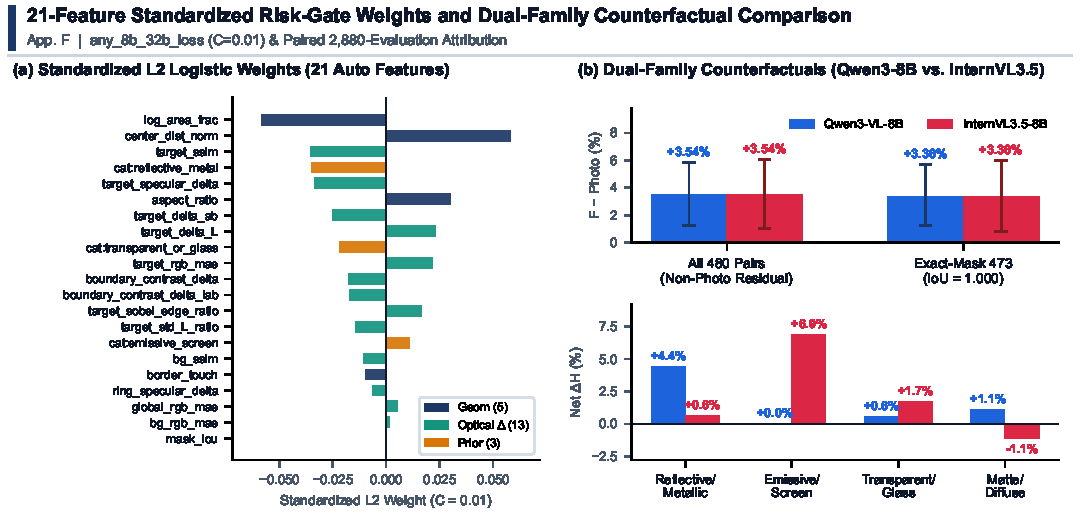
\includegraphics[width=0.97\textwidth]{app_fig5_features_and_counterfactuals.pdf}
\caption{\textbf{Full 21-feature standardized risk-gate coefficients and dual-family counterfactual residual invariance.}
\emph{(a)} Standardized $\ell_2$ logistic regression weights ($C{=}0.01$) predicting family-calibrated \textsc{Qwen3-VL} regressions (\texttt{any\_8b\_32b\_loss}), separated into simulator mask geometry (5 cues), paired appearance/edge deltas (13 cues), and coarse category priors (3 cues).
\emph{(b)} Side-by-side comparison across \textsc{Qwen3-VL-8B} and \textsc{InternVL3.5-8B-HF}: identical $+3.54\%$ ($+3.38\%$ on bit-identical masks) non-photometric \textsc{BSDF} residual above $\mathrm{CIE}~L^*a^*b^*$ matching alongside diverging regime gains.}
\label{fig:app-features-cf}
\end{figure*}

\subsection{Cross-family counterfactual invariance and mask-support sensitivity}
Table~\ref{tab:app-counterfactual-dual} and Figure~\ref{fig:app-features-cf}(b) expand Section~\ref{sec:mechanisms} with full confidence intervals across all $2{,}880$ counterfactual evaluations (\textsc{Qwen3-VL-8B} and \textsc{InternVL3.5-8B-HF}). Although \textsc{InternVL3.5-8B-HF} starts from slightly higher baseline photometric sensitivity ($7.08\%$ vs.\ $5.83\%$ flip rate on $I^{\text{photo}}$) and full conversion turnover ($10.62\%$ vs.\ $9.38\%$), subtracting the $\mathrm{CIE}~L^*a^*b^*$-matched luminance/chromatic control reveals an identical \textbf{$+3.54\%$ non-photometric shader residual} ($[+1.25\%, +5.83\%]$ and $[+1.04\%, +6.04\%]$). Restricting the comparison to the $473/480$ pairs with bit-identical simulator masks ($\mathrm{IoU}{=}1.000$) yields virtually unchanged residuals of \textbf{$+3.38\%$} on both architectures ($[+1.26\%, +5.70\%]$ and $[+0.84\%, +5.97\%]$), confirming that silhouette boundary anti-aliasing on the remaining $7$ pairs does not confound the optical finding. Under objective pixel-distortion grouping (Panel~C), \emph{Low-Distortion} targets gain $+3.76\%$ (\textsc{Qwen3}) and $+3.01\%$ (\textsc{InternVL3.5}), whereas heavily \emph{Specular-Stripped} targets suffer $-7.14\%$ net drop on \textsc{Qwen3-VL-8B}.

\begin{table*}[!t]
\centering
\caption{Complete 21-feature zero-\textsc{VLM} risk-gate inventory (\texttt{deploy\_auto}), reporting group membership, mean $\pm$ SD stratified by \textsc{Qwen3-VL} regression status (\texttt{any\_8b\_32b\_loss}: $455$ non-loss vs.\ $25$ loss pairs), direction-aligned univariate \textsc{AUROC}, and fitted standardized $\ell_2$ weights ($C{=}0.01$).}
\label{tab:app-features21}
\resizebox{\textwidth}{!}{% Generated automatically by build_cviu_appendix_assets.py from pair_optical_features.json & risk_auditor.json
\begin{tabular}{@{}llrrrr@{}}
\toprule
Feature Name & Definition & No-Loss ($n{=}455$) & Loss ($n{=}25$) & Univar.\ AUROC & $\ell_2$ Weight $w_j$ \\
\midrule
\multicolumn{6}{@{}l}{\textit{Simulator Mask Geometry (5)}} \\
\texttt{log\_area\_frac} & Logarithm of target pixel area fraction & -2.432 $\pm$ 0.921 & -2.888 $\pm$ 0.890 & 0.665 & -0.0585 \\
\texttt{aspect\_ratio} & Target bounding-box width-to-height ratio & 1.270 $\pm$ 1.122 & 1.561 $\pm$ 1.194 & 0.560 & +0.0303 \\
\texttt{center\_dist\_norm} & Euclidean distance from frame center (normalized) & 0.331 $\pm$ 0.058 & 0.378 $\pm$ 0.063 & 0.703 & +0.0584 \\
\texttt{border\_touch} & Indicator whether target bbox touches image border & 0.020 $\pm$ 0.139 & 0.000 $\pm$ 0.000 & 0.510 & -0.0097 \\
\texttt{mask\_iou} & Mask overlap IoU between original and converted captures & 0.998 $\pm$ 0.026 & 1.000 $\pm$ 0.000 & 0.508 & +0.0000 \\
\midrule
\multicolumn{6}{@{}l}{\textit{Paired Optical, Chromatic \& Structural Deltas (13)}} \\
\texttt{global\_rgb\_mae} & Full-frame mean absolute RGB difference & 0.110 $\pm$ 0.048 & 0.120 $\pm$ 0.072 & 0.510 & +0.0053 \\
\texttt{target\_rgb\_mae} & Target-mask mean absolute RGB difference & 0.126 $\pm$ 0.094 & 0.193 $\pm$ 0.180 & 0.577 & +0.0216 \\
\texttt{bg\_rgb\_mae} & Background mean absolute RGB difference & 0.108 $\pm$ 0.047 & 0.114 $\pm$ 0.076 & 0.549 & +0.0017 \\
\texttt{target\_delta\_L} & Mean target lightness shift $|\Delta L^*|$ & 8.866 $\pm$ 9.387 & 16.134 $\pm$ 19.356 & 0.566 & +0.0229 \\
\texttt{target\_delta\_ab} & Mean target chromatic shift $\|\Delta(a^*, b^*)\|_2$ & 1.122 $\pm$ 1.742 & 0.801 $\pm$ 1.142 & 0.568 & -0.0248 \\
\texttt{target\_std\_L\_ratio} & Converted-to-original lightness std ratio on target & 1.048 $\pm$ 0.573 & 1.055 $\pm$ 0.428 & 0.515 & -0.0142 \\
\texttt{target\_ssim} & Local $8{\times}8$ structural similarity inside target & 0.652 $\pm$ 0.207 & 0.560 $\pm$ 0.221 & 0.618 & -0.0353 \\
\texttt{bg\_ssim} & Local $8{\times}8$ structural similarity on background & 0.762 $\pm$ 0.120 & 0.763 $\pm$ 0.122 & 0.506 & -0.0104 \\
\texttt{target\_sobel\_edge\_ratio} & Converted-to-original Sobel $|\nabla L^*|$ ratio on target & 0.957 $\pm$ 0.775 & 0.941 $\pm$ 0.430 & 0.505 & +0.0164 \\
\texttt{target\_specular\_delta} & Highlight pixel ($Y>0.88$) fraction shift on target & 0.008 $\pm$ 0.086 & -0.013 $\pm$ 0.193 & 0.514 & -0.0333 \\
\texttt{ring\_specular\_delta} & 12-px exterior ring specular fraction shift & 0.001 $\pm$ 0.034 & 0.014 $\pm$ 0.056 & 0.558 & -0.0063 \\
\texttt{boundary\_contrast\_delta} & 8-px inner/outer contour lightness contrast shift & -0.445 $\pm$ 8.405 & -5.479 $\pm$ 13.232 & 0.623 & -0.0176 \\
\texttt{boundary\_contrast\_delta\_lab} & 8-px inner/outer contour $\mathrm{CIE}~\Delta E_{ab}^*$ shift & -0.621 $\pm$ 8.225 & -5.452 $\pm$ 13.202 & 0.615 & -0.0169 \\
\midrule
\multicolumn{6}{@{}l}{\textit{Coarse Target Category Priors (3)}} \\
\texttt{cat\_is\_transparent\_or\_glass} & Transparent/glass object category prior & 0.070 $\pm$ 0.256 & 0.000 $\pm$ 0.000 & 0.535 & -0.0220 \\
\texttt{cat\_is\_reflective\_appliance\_or\_metal} & Reflective appliance/metal category prior & 0.402 $\pm$ 0.490 & 0.440 $\pm$ 0.496 & 0.519 & -0.0348 \\
\texttt{cat\_is\_emissive\_or\_screen} & Emissive/screen category prior & 0.185 $\pm$ 0.388 & 0.160 $\pm$ 0.367 & 0.512 & +0.0109 \\
\bottomrule
\end{tabular}
}
\end{table*}

\subsection{Per-feature breakdown of the 21-cue zero-VLM risk gate}
Table~\ref{tab:app-features21} and Figure~\ref{fig:app-features-cf}(a) dissect why lightweight pre-deployment risk gating achieves $0.743$ test \textsc{AUROC} ($0.732$ 30-scene \textsc{LOSO} with \texttt{geometry\_only}, catching $52.0\%$ of regressions in the top $20\%$ triage budget) while global \textsc{RGB MAE} fails ($0.432$ test \textsc{AUROC}). Regression targets are systematically smaller (\texttt{log\_area\_frac}: $-2.888$ vs.\ $-2.432$, weight $-0.0585$), positioned closer to frame peripheries (\texttt{center\_dist\_norm}: $0.378$ vs.\ $0.331$, univariate \textsc{AUROC} $= 0.703$, weight $+0.0584$), and undergo stronger local structural degradation inside the target mask (\texttt{target\_ssim}: $0.560$ vs.\ $0.652$, weight $-0.0353$) alongside negative boundary contrast shifts (\texttt{boundary\_contrast\_delta}: $-5.479$ vs.\ $-0.445$, univariate \textsc{AUROC} $= 0.623$). By contrast, \texttt{global\_rgb\_mae} carries near-random univariate separability ($0.510$) because global metallic reflections inflate pixel differences on easy scenes where glare removal improves grounding.

\section{Navigation Outcomes, Runtime Checks, and Trajectory Cases}
\label{app:navigation}

\begin{figure*}[!t]
\centering
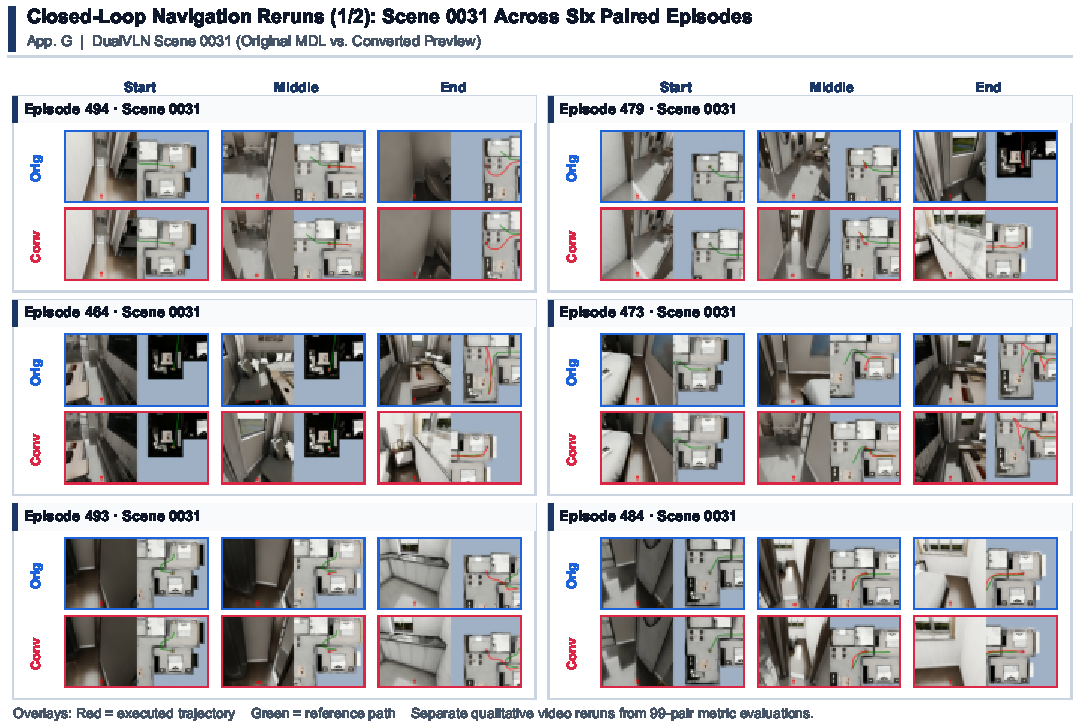
\includegraphics[width=0.86\textwidth]{app_fig6_nav_plate1.pdf}
\caption{\textbf{Consolidated closed-loop navigation reruns (1/2): \textsc{KuJiaLe Scene 0031}.}
Six paired episode recordings comparing \original{} (\textsc{MDL}) against \converted{} (\usdps{}) across \emph{Start}, \emph{Middle}, and \emph{End} frames with top-down occupancy maps (red: executed route; green: reference path). Recordings are separate qualitative reruns sharing episode IDs with the 99-pair metric benchmark.}
\label{fig:app-navcases1}
\end{figure*}

To examine how individual trajectory metrics co-vary under shader lowering, we inspect the full closed-loop evaluation across 99 paired episode IDs spanning \textsc{KuJiaLe} scenes \texttt{0031}, \texttt{0036}, and \texttt{0066} ($33$ episodes per scene), holding language instructions, start states, and policy weights fixed across \original{} and \converted{}. Table~\ref{tab:app-navfull} adds oracle success, step counts, fall/stuck fractions, and 95\% paired bootstrap confidence intervals to the main summary: aggregate \textsc{SR} ($-4.04$~pp), \textsc{SPL} ($-4.41$~pp), and oracle success ($-5.05$~pp) shift modestly while $30/99$ episodes reverse binary pass/fail outcomes ($17$ success-to-failure, $13$ failure-to-success) alongside an increase of $+41.75$ mean action steps. Separate fresh-launch simulator checks ($9$ loads per condition across all $3$ scenes; Table~\ref{tab:app-navload}) verify comparable initialization time ($13.95\,\mathrm{s}$ vs.\ $14.12\,\mathrm{s}$), warm-up frame rate ($2.36$ vs.\ $2.42\,\mathrm{FPS}$), and GPU footprint ($3{,}807$ vs.\ $3{,}829\,\mathrm{MB}$).

\begin{table*}[!t]
\centering\scriptsize
\begin{minipage}[t]{0.49\textwidth}
\centering
\setlength{\tabcolsep}{4pt}
\resizebox{\linewidth}{!}{% Generated by appendix/build_tables.py; source hashes in table_sources.json.
\begin{tabular}{lrrrr}
\toprule
Metric & Original & Converted & $\Delta$ & 95\% paired CI \\
\midrule
SR (\%) & 52.530 & 48.480 & -4.040 & [-15.150, 7.070] \\
SPL (\%) & 47.390 & 42.980 & -4.410 & [-14.170, 5.140] \\
Oracle success (\%) & 66.670 & 61.620 & -5.050 & [-15.150, 5.050] \\
Navigation error & 3.680 & 3.631 & -0.049 & [-0.646, 0.539] \\
Trajectory length & 6.975 & 7.060 & +0.084 & [-0.737, 0.930] \\
Action steps & 233.647 & 275.394 & +41.748 & --- \\
Fall rate & 0.020 & 0.020 & +0.000 & --- \\
Stuck rate & 0.000 & 0.000 & +0.000 & --- \\
\bottomrule
\end{tabular}
}
\caption{Full closed-loop navigation metrics across all 99 paired \textsc{DualVLN} episodes (differences reported as \converted{} minus \original{}, with 95\% paired bootstrap CIs where retained).}
\label{tab:app-navfull}
\end{minipage}\hfill
\begin{minipage}[t]{0.48\textwidth}
\centering
\setlength{\tabcolsep}{3pt}
\resizebox{\linewidth}{!}{% Generated by appendix/build_tables.py; source hashes in table_sources.json.
\begin{tabular}{lrrrr}
\toprule
Condition & Loads & Ready time (s) & Warm-up FPS & GPU memory (MB) \\
\midrule
Original & 9/9 & 13.95 [11.64, 16.28] & 2.36 [2.01, 2.70] & 3807 [3748, 3862] \\
Converted & 9/9 & 14.12 [12.31, 16.24] & 2.42 [2.08, 2.73] & 3829 [3689, 3971] \\
\bottomrule
\end{tabular}
}
\caption{Fresh-launch simulator initialization, frame rate, and GPU memory checks ($9$ runs per condition across scenes \texttt{0031}, \texttt{0036}, and \texttt{0066}).}
\label{tab:app-navload}
\end{minipage}
\end{table*}

\begin{figure*}[!t]
\centering
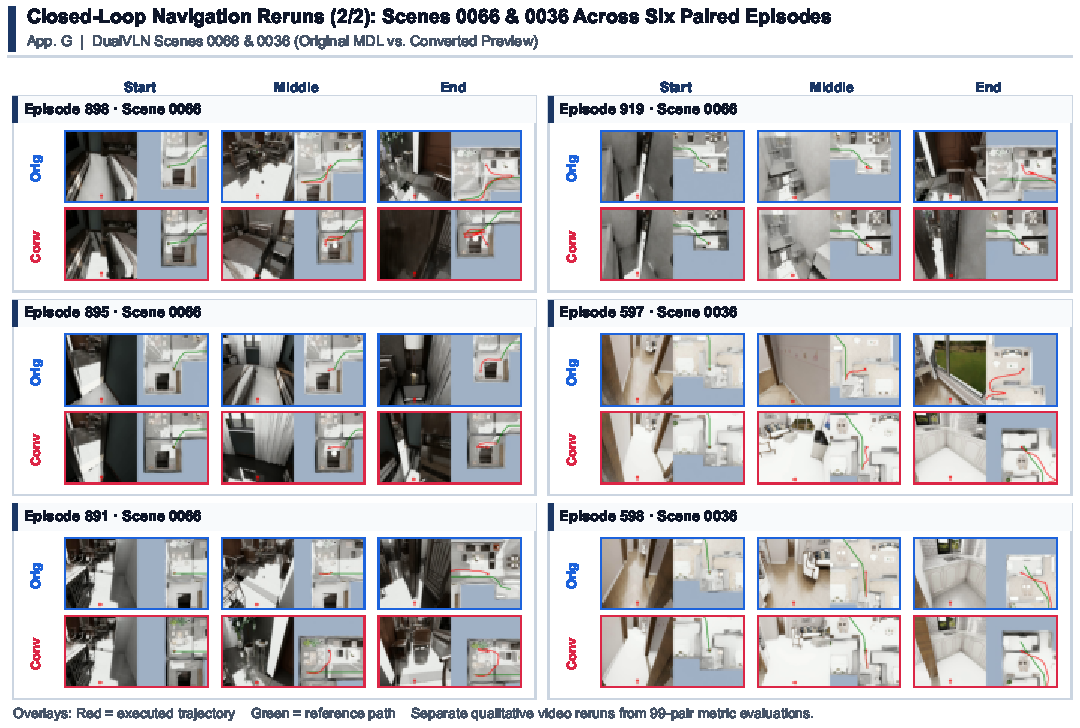
\includegraphics[width=0.84\textwidth]{app_fig7_nav_plate2.pdf}
\caption{\textbf{Consolidated closed-loop navigation reruns (2/2): \textsc{KuJiaLe Scenes 0066 \& 0036}.}
Six paired episode recordings from scenes \texttt{0066} and \texttt{0036} matching the layout of Figure~\ref{fig:app-navcases1}. Minor shader-induced observation shifts can trigger divergent room-entry timing and early termination even on shared start states and instructions.}
\label{fig:app-navcases2}
\end{figure*}

\subsection{Twelve paired recorded trajectory examples}
Figures~\ref{fig:app-navcases1} and~\ref{fig:app-navcases2} consolidate all 12 qualitative video reruns into two panoramic plates across all three scenes, covering asymmetric failures, divergent trajectories sharing identical final binary status, and consistent routes. For example, in episode~898 (scene~\texttt{0066}), the converted rollout loops near the entryway while the original rollout reaches deeper rooms; in episode~891, the converted agent takes a wide kitchen detour; whereas episode~598 terminates near matched kitchen viewpoints under both shaders. Because each metric rollout executed a single closed-loop trajectory per shader condition, these episode outcomes reflect both shader shifts and single-rollout controller dynamics.

\section{Implementation and Reproducibility Details}
\label{app:reproduction}

\subsection{Model Execution Environment}
All primary static-grounding, variance-control, and counterfactual evaluations run in unquantized \texttt{torch.bfloat16} precision (\texttt{device\_map="auto"}) using \texttt{transformers 5.23.0} on an NVIDIA RTX~4090 (24\,GB) GPU across four open-weight \textsc{VLM} families (six checkpoints, 14,016 evaluations total): \textsc{Qwen3-VL-2B/8B/32B}, \textsc{InternVL3.5-8B-HF}, \textsc{Molmo2-8B}, and \textsc{LLaVA-NeXT-Mistral-7B}. Deterministic runs use greedy decoding ($T{=}0$, \texttt{do\_sample=False}) with a 64--128 max-new-token generation budget; the \textsc{Qwen3-VL-8B} stochastic control evaluates five draws at $T{=}0.2$ and $\text{top-}p{=}0.95$. Closed-loop \textsc{InternNav/DualVLN} evaluations and simulator initialization checks run under identical scene graphs, start poses, episode limits, and policy weights between \original{} and \converted{}.

\subsection{Counterfactual Compositing and Risk-Gate Training}
For photometric matching ($I_i^{\text{photo}}$), RGB values are transformed to $\mathrm{CIE}~L^*a^*b^*$ under D65 sRGB calibration, and each channel is linearly matched in mean and standard deviation toward $I_i^C$ independently inside the simulator target mask $M_i^O$ and inside the background complement before clipping to valid $[0, 255]$ RGB integers. Target-only ($I_i^T$) and background-only ($I_i^B$) composites apply symmetric boundary union handling across the 7/480 pairs with anti-aliased thin-rim mask differences ($\mathrm{IoU} \ge 0.96$). All 95\% confidence intervals and paired contrasts draw 10,000 bootstrap replicates resampled over whole scene clusters ($S{=}30$). For zero-\textsc{VLM} risk gating, all 21 continuous features are standardized using training-split statistics only (15 scenes, $n{=}240$); $\ell_2$-regularized logistic regression selects regularization strength $C \in \{0.01, 0.1, 1.0, 10.0\}$ on the validation scenes ($n{=}80$) before evaluating on held-out test scenes ($n{=}160$) and 30-scene \textsc{LOSO} folds ($n{=}480$).

\subsection{Asset Provenance and Licensing}
\balance
Indoor 3D environments originate from the SimReady \textsc{GRScenes} benchmark and \textsc{KuJiaLe} apartment scenes, paired with open-weight \textsc{VLM} checkpoints from Hugging Face and ModelScope under their respective academic licenses. Paired renders, segmentation masks, and analysis scripts will be released publicly upon publication to support exact replication of all quantitative tables and figures.


\end{document}
